\chapter{Dissipation of primordial perturbations}\label{chap:dissipation}
\label{sec:dissipation_PGW}
Primordial perturbations, when reentering the Hubble horizon after inflation, excite standing waves (e.g. of temperature) in the plasma that, depending on the phase of the wave, lead to different patches of photons to be hotter or colder than the average. Later on, these photons can diffuse in the baryon-photon plasma and mix together. In this way, diffusion dissipates the standing waves and generates distortions in the \emph{CMB spectrum}. For scalar perturbations, this well known effect is called \emph{Silk damping}. The same phenomenon takes place also for primordial gravitational waves, however, due to the different physics of tensor perturbation compared to scalar ones, the sourcing mechanism has some differences. In particular, gravitational waves dissipates at a slower rate than scalar perturbations and they are in general weaker, leading to smaller amplitudes, but they are sourced by a broader spectrum of modes. In this chapter we will study in depth this processes to determine the heating rate associated to them.

\section{Mixing of blackbodies}\label{sec:MixingOfBlackbodies}
The \textbf{mixing of blackbodies} at different temperatures (by diffusion) is a two steps process.
Initially, it produces \emph{y-distortions}, then in the $\mu$-era \textbf{comptonization} brings the equilibrium phase space distribution to a Bose-Einstein one (see Section \ref{sec:ThermalizationProblem}), turning the initial distortions in \emph{$\mu$-distortions}. In the following sections we will describe these two processes in detail.

\subsection{From blackbodies to y-distortions}
We already discovered that at high redshifts all the interactions in the primordial plasma bring the photons to a state of thermal equilibrium described by the Planck distribution
$$B(\nu,T)=\frac{1}{\exp[\nu/(k_BT_e)]-1}=\big(e^x-1\big)^{-1},\qquad \text{with }x=\frac{\nu}{k_BT_e}.$$
From this distribution we can evaluate the number density and the energy density of the photons in the radiation (see Section \ref{sec:thdm_obs})
\begin{align*}
    n=b_RT^3,\qquad \rho=a_RT^4,
\end{align*}
where $a_R\defeq\pi^2k_B^4/15$ and $b_R\defeq 2k_B^3\zeta(3)/\pi^2$, with the number of internal degrees of freedom of photons $g_\text{dof}=2$.\\From the first principle of thermodynamics and choosing as the intensive thermodynamic variable $T$, we can then obtain the entropy density ($s=S/V$) by
\begin{align*}
    TdS&=TVds+Ts\ dV=TV\frac{\partial s}{\partial T}\bigg|_V dT+Ts\ dV\\&=d(\rho V)+PdV=Vd\rho+\rho\ dV+PdV=V\frac{\partial \rho}{\partial T}\bigg|_V dT+\rho\ dV+\frac{1}{3}\rho\ dV\\\Rightarrow& \quad \bigg(TV\frac{\partial s}{\partial T}\bigg|_V-V\frac{\partial \rho}{\partial T}\bigg|_V\bigg)dT=\bigg(\frac{4}{3}\rho+Ts\bigg)dV\quad\Rightarrow\quad \boxed{s=\frac{4}{3}\frac{\rho}{T}=\frac{4}{3}a_RT^3},
\end{align*}
where we used the equation of state for radiation $P=\frac{1}{3}\rho$ and the fact that the change of temperature and volume must be independent.

Zeldovich \cite{Zeldovich1972} showed that in general a mixing of blackbody spectra results in the appearance of a y-distortion. This can easily be understood by Taylor expanding a Planck distribution whose temperature depends on the position in the plasma (so that this describes a different blackbody spectrum at each point in space) and then taking the spatial average. This can also be seen as an ensemble of blackbodies at different temperatures, for which the average becomes an ensemble average. Considering a temperature $\bar{T}+\Delta T(x)$, with $\Delta T\ll\bar{T}$ the expansion of $B\big[x/(1+\Delta T/\bar T)\big]$ would result in a temperature shift (see Section\ref{eq:SD_temperature_shift}). However, this kind of distortion, being linear in $\Delta T/\bar T$, will give no distortion terms after the spatial average (hotter and colder spots, on average, give the mean temperature $\bar T$). A temperature shift expanded at the second order (equation \eqref{eq:SD_2ord_temp_shift}) instead gives rise to non-vanishing terms in the average
\begin{align}
     \nonumber\bigg\langle B\bigg(\frac{x}{1+(\Delta T/\bar T)^2}\bigg)\bigg\rangle&\approx\bigg\langle B(x)+G(x)\frac{\Delta T}{\bar T}+\frac{1}{2}\big[Y(x)+2G(x)\big]\bigg(\frac{\Delta T}{\bar T}\bigg)\bigg\rangle\\\nonumber
     &=B(x)+G(x)\bigg\langle\frac{\Delta T}{\bar T}\bigg\rangle+\frac{1}{2}\big[Y(x)+2G(x)\big]\bigg\langle\bigg(\frac{\Delta T}{\bar T}\bigg)^2\bigg\rangle\\&\bigg\downarrow \bigg\langle\frac{\Delta T}{\bar T}\bigg\rangle=0,\ B(x)+G(x)\bigg\langle\bigg(\frac{\Delta T}{\bar T}\bigg)^2\bigg\rangle\approx B\bigg(\frac{x}{1+\big\langle(\Delta T/\bar T)^2\big\rangle}\bigg),\nonumber\\
     &\approx B\bigg(\frac{x}{1+\big\langle(\Delta T/\bar T)^2\big\rangle}\bigg)+\frac{1}{2}Y(x)\bigg\langle\bigg(\frac{\Delta T}{\bar T}\bigg)^2\bigg\rangle,\label{eq:Mixing_Y_SD}
\end{align}
where we used that the mean of the temperature perturbations is zero, and we recognized a first order temperature shift distortion in the term proportional to $G(x)$.\\ The above calculation thus shows that the mixing of blackbodies, not only results in a y-distortion, but also in a small increase in temperature to $T_{\text{new}}=\bar T(1+\langle(\Delta T/\bar T)^2\rangle)$. We shall also recall that a y-distortion maintains unchanged the number of photons in the radiation: indeed the mixing consists just in a spatial redistribution of "hotter" and "colder" photons. Hence, even though the temperature increases and thus one should expect a change in the number of photons, this happens only with respect to the number density of each blackbody, while the total number of photons remains unchanged.

Another way to see this phenomenon is by considering directly the mixing of two blackbodies at temperature $T_1=\bar T+\Delta T$ and $T_2=\bar T-\Delta T$ (now $\Delta T$ is not a function of space anymore). Before the two blackbodies have mixed, a fraction of photons  obey the first blackbody distribution while some others the second one\footnote{Approximately half are at $T_1$ and the other half at $T_2$ since the two temperatures are really close.}: hence the initial energy density, number density and entropy density are just the average of the two blackbodies:
\begin{align}\label{eq:Mix_rho_initial}
    \rho_\text{initial}&= \frac{1}{2}a_R(T_1^4+T_2^4)\approx a_R\bar T^4\bigg[1+6\bigg(\frac{\Delta T}{\bar T}\bigg)^2\bigg]>a_R\bar T^4,\\\label{eq:Mix_n_initial}
    n_\text{initial}&= \frac{1}{2}b_R(T_1^3+T_2^3)\approx b_R\bar T^3\bigg[1+3\bigg(\frac{\Delta T}{\bar T}\bigg)^2\bigg]>b_R\bar T^3,\\\label{eq:Mix_s_initial}
    s_\text{initial}&= \frac{1}{2}\frac{4}{3}a_R( T_1^3+T_2^3)\approx\frac{4}{3}a_R\bigg[1+3\bigg(\frac{\Delta T}{\bar T}\bigg)^2\bigg]>\frac{4}{3}a_R\bar T^3,
\end{align}
where for each quantity we Taylor expanded for $\Delta T/\bar T\ll 1$ at the first order.\\
Note that all the three averages are larger than the densities that would have a single blackbody at the average temperature $\bar T$. These extra contributions, as we will see, are responsible for the creation of the distortions.\\After the mixing, there will be a single blackbody spectrum (plus distortions) with a new temperature $T_\text{final}$; since the number of photons is unchanged (we only mix them) we can obtain this new temperature from the initial number density using $n=b_RT^4$ for blackbodies
$$T_\text{final}=\bigg(\frac{n_\text{initial}}{b_R}\bigg)^{1/3}\approx\bar T\bigg[1+\bigg(\frac{\Delta T}{\bar T}\bigg)^2\bigg],$$ similarly to what we found with the previous approach. The extra photons thus cause only an increase in the temperature because the y-distortion conserves the number of photons ($\int dx\ x^2Y(x)=0$), hence only the blackbody part of the spectrum and the temperature shift, from the \eqref{eq:Mixing_Y_SD}, contribute to the number density.\\
Now, the final temperature allows us to evaluate the final energy density
$$\rho_\text{final}=a_RT_\text{final}^4\approx a_R\bar T^4\bigg[1+4\bigg(\frac{\Delta T}{\bar T}\bigg)^2\bigg]<\rho_\text{initial},$$ which we find to be smaller that the initial one. This is because some energy is now stored in the form of the y-distortion (that we haven't considered yet since we are only using the observable of a blackbody). Indeed, by comparing $\rho-a_R\bar T^4$, which (form equation \ref{eq:Mixing_Y_SD}) is the energy density associated to all the distortions (temperature shift + y-distortion), we discover that only $2/3$ of this energy is then transferred in the new blackbody radiation at $T_\text{final}$ (in the form of the temperature shift)
$$\rho_\text{final}-a_R \bar T^4=4\bigg(\frac{\Delta T}{\bar T}\bigg)^2a_R\bar T^4=\frac{2}{3}\bigg(\rho_\text{initial}-a_R \bar T^4\bigg).$$
The remaining $1/3$ of the energy corresponds to the contribution of the y-distortion
$$\frac{1}{3}\bigg(\rho_\text{initial}-a_R \bar T^4\bigg)=2\bigg(\frac{\Delta T}{\bar T}\bigg)^2a_R\bar T^4\propto\frac{1}{2}\bigg(\frac{\Delta T}{\bar T}\bigg)^2\int dx\ x^3 Y(x).$$
Lastly, we can compute the final entropy density$$ s_\text{final}=\frac{4}{3}a_RT_\text{final}^3\approx\frac{4}{3}a_R \bar T^4\bigg[1+3\bigg(\frac{\Delta T}{\bar T}\bigg)^2\bigg]=s_\text{initial}.$$ This holds only for the entropy associated to the new shifted blackbody spectrum as also the y-distortion should contribute to it. We can compute this last contribution from the fraction of energy stored in the y-distortion $\Delta \rho = (\rho_\text{initial}-a_R \bar T^4)/3$
$$\Delta s=\frac{\Delta \rho}{T}\approx 2a_R \bar T^3\bigg(\frac{\Delta T}{\bar T}\bigg)^2.$$
Note that this must be expected since, when mixing two blackbodies the entropy should increase as when we mix two fluids, hence the initial entropy cannot be the same as the final.

To sum up what we discovered, mixing of blackbodies leads to a new spectrum that can be decomposed in two parts: a blackbody at a higher temperature $T_\text{new}=\bar T\big(1+\langle(\Delta T/\bar T)^2\rangle\big)$ and a y-distortion. While the number of photons is conserved (since we are only mixing them) and fully accounted by the blackbody part, the energy and entropy are redistributed between the temperature shift of the blackbody and the y-distortion. Exactly, $2/3$ of the energy associated to the distortions is directly transferred to the new blackbody (as a temperature increase), while the remaining $1/3$ is stored in the y-distortion. The entropy associated with the blackbody is instead conserved, while a new contribution appears due to the y-distortion. We shall indicate that, although part of our calculations used only the mixing of two blackbodies, considering an ensemble of $n$ blackbodies the result can be generalized without spoiling our solution. Indeed, it is sufficient to replace $(\Delta T/\bar T)^2$ by $\langle(\Delta T/\bar T)^2\rangle$ to account for the whole ensemble, as explained in \cite{MixingBB}.
\subsection{Comptonization of mixed blackbodies}
\label{sec:MixSD_Comportonization}
The previously described mixing of blackbodies does not take into consideration the interactions in the plasma, this means that a y-distortion is produced at redshifts $z<z_{\mu y}\approx 5\times 10^4$ (see Section \ref{sec:ThermalizationProblem}). Compton scattering instead thermalizes the radiation to a Bose-Einstein distribution (or a Planckian if also Bremsstrahlung and double Compton scattering are efficient). We will show that during the $\mu$-era thermal processes convert y-distortions into $\mu$-distortions. 

To obtain the amplitude of the new distortion generated we can proceed to consider the mixing of the two previously introduced blackbodies, respectively at $T_1$ and $T_2$. We assume that after comptonization the temperature of the radiation changes from $T_\text{new}=\bar T\big[1+(\Delta T/\bar T)^2\big]$ to $T_\text{BE}=T_\text{new}(1+t_\text{BE})\approx\bar T\big[+t_\text{BE}+(\Delta T/\bar T)^2\big]$, where $t_\text{BE}\ll1$ measures this change of temperature. 
Now, the energy and number densities are fully described by the Bose-Einstein distribution, in Appendix \ref{sec:SmallChemicalPotential} approximated formulae for these are obtained in the limit of small chemical potential. Since comptonization conserves the number of photons (in Section \ref{sec:ThermalizationProblem} we discussed that no extra photons are created by Compton scattering) we can compare the initial number density to the final one. Then, since the blackbodies are at very close temperatures, we can assume that they are almost in thermal equilibrium with the other components of the plasma. Hence, the exchange of energy between different species of the plasma is negligible and we can consider the energy density of the photons unchanged. In this way, Compton scattering redistributes the energy of photons using electrons as mediators. Using equation \eqref{eq:SmallChemicalPotential_n} and \eqref{eq:SmallChemicalPotential_rho} we can equate the initial and final number and energy densities:
\begin{align*}
    n_\text{final}&\approx b_R T^3_\text{BE}\bigg(1-\mu\frac{\zeta(2)}{\zeta(3)}\bigg)\approx b_R \bar T^3\bigg(1+3t_\text{BE}+3\bigg(\frac{\Delta T}{\bar T}\bigg)^2-\mu\frac{\zeta(2)}{\zeta(3)}\bigg)\\
    &=n_\text{initial}=b_R\bar T^3\bigg[1+3\bigg(\frac{\Delta T}{\bar T}\bigg)^2\bigg],\\
    \rho_\text{final}&\approx b_R T^4_\text{BE}\bigg(1-\mu\frac{\zeta(3)}{\zeta(4)}\bigg)\approx b_R \bar T^3\bigg(1+4t_\text{BE}+4\bigg(\frac{\Delta T}{\bar T}\bigg)^2-\mu\frac{\zeta(3)}{\zeta(4)}\bigg)\\
    &=\rho_\text{initial}=b_R\bar T^3\bigg[1+6\bigg(\frac{\Delta T}{\bar T}\bigg)^2\bigg].
\end{align*}
From the first equation we obtain that $t_\text{BE}= \mu{\zeta(2)}/{3\zeta(3)}$, inserting this relation in the second equation we get
\begin{align}
    \mu&=2\bigg(\frac{4\zeta(2)}{3\zeta(3)}-\frac{\zeta(3)}{\zeta(4)}\bigg)^{-1}\bigg(\frac{\Delta T}{\bar T}\bigg)^2\approx2.802\bigg(\frac{\Delta T}{\bar T}\bigg)^2,\label{eq:mu_MixingBB}\\
    t_\text{BE}&=\frac{2\zeta(2)}{3\zeta(3)}\bigg(\frac{4\zeta(2)}{3\zeta(3)}-\frac{\zeta(3)}{\zeta(4)}\bigg)^{-1}\bigg(\frac{\Delta T}{\bar T}\bigg)^2\approx1.278\bigg(\frac{\Delta T}{\bar T}\bigg)^2.\label{eq:t_BE_MixingBB}
\end{align}
Note that the same chemical potential can be obtained by considering a that all the energy stored in the y-distortion gets transferred to the $\mu$-distortion, using equation \eqref{eq:SD_mu_amplitude}:$$\mu=1.401\frac{\Delta \rho}{\rho}=1.401\frac{\frac{1}{3}(\rho_\text{initial}-a_R \bar T^4)}{a_R \bar T^4}=1.401\times\frac{6}{3}\bigg(\frac{\Delta T}{\bar T}\bigg)^2=2.802\bigg(\frac{\Delta T}{\bar T}\bigg)^2.$$
To conclude, let us write the total spectral distortion that we obtain after comptonization:
$$f(x)=B(x)+G(x)\bigg[\bigg(\frac{\Delta T}{\bar T}\bigg)^2+t_\text{BE}\bigg]-\mu\frac{G(x)}{x},$$
where, after the Planckian spectrum $B$, we have the total temperature shift (both from the mixing and the comptonization) and the $\mu$-distortion. Note that the latter appears as $-G(x)/x$ and not at as $M(x)$: this is because we assumed that the temperature changes during comptonization and then we imposed that the number of photons is conserved. Hence, the temperature shift $t_\text{BE}$ already accounts also for the shift that would be contained in $M$.

Again, this result can be generalized to the case of mixing $n$ blackbodies by replacing the factors $(\Delta T /\bar T)^2$ with the ensemble average $\langle(\Delta T /\bar T)^2\rangle$.

\subsection{Mixing of polarized blackbodies}
\label{sec:MixingPolarization}
In our discussion of the mixing of blackbodies we still haven't taken into account also that the radiation is polarized. To connect to Section \ref{sec:ComptonPolarization} we shall change our notation to be consistent to the usual definition of \emph{CMB anisotropies} $\Theta(x,t)\defeq \Delta T/\bar T$.

We start by describing linearly polarized light, then the more general case will be deduced exploiting the following calculations. We start by introducing the \emph{phase space matrix}
\begin{equation*}
    \mathcal{F} _\text{unpol} \defeq
    \begin{pmatrix}
        B(x) & 0 \\ 0 & B(x)
    \end{pmatrix}\ \xrightarrow{\text{polarization}}\mathcal{F}  \defeq
    \begin{pmatrix}
        B\big(x/[1+\Theta_\parallel]\big) & 0 \\ 0 & B\big(x/[1+\Theta_\perp ]\big)
    \end{pmatrix},
\end{equation*}
where $\Theta_\perp$ and $\Theta_\parallel$ are the temperature fluctuations associated to photons that are polarized either in the perpendicular direction or in the orthogonal one and $B(x)$ is the Planckian spectrum. The total phase space distribution is then recovered by taking the trace of the above matrices $f=\text{Tr}(\mathcal{F} )/2$, which corresponds to the average of the two polarizations.\\
It is useful to rewrite the above in terms of the \emph{ Pauli matrices} $\sigma_i$
$$\mathcal{F} =\frac{f_\parallel+f_\perp}{2}\begin{pmatrix}
    1&0\\0&1
\end{pmatrix}+\frac{f_\parallel-f_\perp}{2}\begin{pmatrix}
    1&0\\0&-1
\end{pmatrix}=f_I\hat 1+f_Q\sigma_3, $$
where $f_\parallel\defeq B\big(x/[1+\Theta_\parallel]\big)$ and $f_\perp\defeq B\big(x/[1+\Theta_\perp]\big)$, while $f_I$ is the distribution associated to the Stokes parameter $I$, and it corresponds to $f$, while $f_Q$ is associated to $Q$.

We can now proceed to expand (as in equation \eqref{eq:Mixing_Y_SD}) the perturbation at the second order to obtain the distortions:
\begin{align*}
    f_I&=\frac{f_\parallel+f_\perp}{2}\approx B(x)+G(x)\frac{\Theta_\parallel+\Theta_\perp+\Theta^2_\parallel+\Theta^2_\perp}{2}+Y(x)\frac{\Theta^2_\parallel+\Theta^2_\perp}{4},\\
    f_Q&=\frac{f_\parallel-f_\perp}{2}\approx G(x)\frac{\Theta_\parallel-\Theta_\perp+\Theta^2_\parallel-\Theta^2_\perp}{2}+Y(x)\frac{\Theta^2_\parallel-\Theta^2_\perp}{4}.
\end{align*}
Now, identifying the right anisotropies associated to each Stokes parameter, $\Theta_I=(\Theta_\parallel+\Theta_\perp)/2$ and $\Theta_Q=(\Theta_\parallel-\Theta_\perp)/2$, we find
\begin{align*}
    f_I&\approx B(x)+G(x)\Big(\Theta_I+\Theta^2_I+\Theta^2_Q\Big)+Y(x)\frac{\Theta^2_I+\Theta^2_Q}{2},\\
    f_Q&\approx G(x)\Big(\Theta_Q+2\Theta_I\Theta_Q\Big)+Y(x)\Theta_I\Theta_Q.
\end{align*}
This shows that also the phase space associated to the $Q$ parameter gets a temperature shift and a y-distortion.

To generalize this result to a generic polarization we can simply consider the phase space distribution $f_U$, by a change of basis this can be rotated into $f_Q$ (as a rotation changes $U\rightarrow Q$). This means that the above calculations holds also for $f_U$ (since the distribution is itself a scalar) and just by rotating everything back we get the final result
\begin{subequations}\label{eq:y-dist_polarization_components}
\begin{align}
    \mathcal{F}=&f_I\hat 1+f_Q\sigma_3+f_U\sigma_1 \\
    f_I&\approx B(x)+G(x)\Big(\Theta_I+\Theta^2_I+\Theta^2_Q+\Theta^2_U\Big)+Y(x)\frac{\Theta^2_I+\Theta^2_Q+\Theta^2_U}{2},\\
    f_Q&\approx G(x)\Big(\Theta_Q+2\Theta_I\Theta_Q\Big)+Y(x)\Theta_I\Theta_Q,\\
    f_U&\approx G(x)\Big(\Theta_U+2\Theta_I\Theta_U\Big)+Y(x)\Theta_I\Theta_U,
\end{align}
\end{subequations}
where we obtained $f_U\sigma_1$ by a change of basis.
The overall y-distortion is given by averaging the phase space distributions 
$$ f\defeq\frac{1}{2}\text{Tr}(\mathcal{F} )= B(x)+G(x)\Big(\Theta_I+\Theta^2_I+\Theta^2_Q+\Theta^2_U\Big)+Y(x)\frac{\Theta^2_I+\Theta^2_Q+\Theta^2_u}{2}$$
and then by taking the spatial average over the temperature anisotropies (recall $\langle\Theta\rangle=0$ as in Section \ref{sec:MixingOfBlackbodies}) 
\begin{align}
    &\langle f\rangle=B(x)+G(x)\Big\langle \Theta^2_I+\Theta^2_Q+\Theta^2_U\Big\rangle+Y(x)\Bigg\langle\frac{\Theta^2_I+\Theta^2_Q+\Theta^2_U}{2}\Bigg\rangle\nonumber\\
    &\Longrightarrow\quad \boxed{y=\frac{1}{2}\Big\langle\Theta^2_I+\Theta^2_Q+\Theta^2_U\Big\rangle}.\label{eq:y-distortion_polarization}
\end{align}
From the above we can integrate the spectral distortion to obtain the energy stored in it: the integral is the same as when we consider unpolarised light from just two blackbodies ($\int dx\ x^3 Y(x)$) but now it is multiplied by $\big\langle\Theta^2_I+\Theta^2_Q+\Theta^2_U\big\rangle$ instead of $(\Delta T/\bar T)^2$. Thus, the final result is that the excess energy of an ensemble of blackbodies at different temperatures reads 
\begin{equation}
    \frac{\Delta \rho}{\rho}\bigg|_\text{excess}=6\Big\langle\Theta^2_I+\Theta^2_Q+\Theta^2_U\Big\rangle,\label{eq:polarize_mixing_excess_energy}
\end{equation}
$1/3$ of this energy generates the y-distortion and the remaining $2/3$ raise the temperature of the radiation.

If Comptonization is still efficient, the y-distortion turns into a $\mu$-distortion. The amplitude of this final distortion can be obtained, as we observed in the previous section, from the \eqref{eq:SD_mu_amplitude} considering that all the energy of the y-distortion is transferred to the $\mu$ one
\begin{equation}
    \label{eq:mu-distortion_polarized}
    \mu=1.401\times\frac{1}{3}\frac{\Delta\rho}{\rho}\bigg|_\text{excess}=2.802\Big\langle\Theta^2_I+\Theta^2_Q+\Theta^2_U\Big\rangle.
\end{equation}

\section{Dissipation of scalar perturbations}
\label{sec:diss_scalar}
We already anticipated that the process of mixing of blackbodies occurs at high redshifts when primordial perturbations reenter the Hubble horizon and start to interact with the plasma. In Section \ref{sec:ThetaTimeEvolution} we studied how the scalar perturbations generate temperature anisotropies as the result of this interaction. Temperature anisotropies, that intuitively we can think as hotter or colder patches of photon plasma, as the universe cools down (the mean free path of photons decreases a little) start to mix. This erases the perturbations at the smallest scales and the dissipated energy produces the spectral distortions. If this process occurs during the $\mu$-era, the resulting distortion is immediately Comptonized and we obtain a $\mu$ distortion, otherwise we are left with the y-distortion.

Equations \eqref{eq:y-distortion_polarization} and \eqref{eq:mu-distortion_polarized} relate the anisotropies in a photon gas to the corresponding y and $\mu$-distortions they can be turned in. However, in the early universe this process is more involved as it happened dynamically as the photon free-streaming scale approaches the scale of the anisotropies. Obtaining the associated heating rate would instead give us a way to connect the dissipation at different redshifts with the thermal history of the plasma to obtain the distortion today. Consider equation \eqref{eq:polarize_mixing_excess_energy}, to consider a dynamical process we can generalize it considering in its right-hand side only the anisotropies that has been dissipated
$$\frac{\Delta\rho}{\rho}\bigg|_{\text{excess}}(t)=6\bigg
(\Big\langle\Theta^2_I(t_0)+\Theta^2_Q(t_0)+\Theta^2_U(t_0)\Big\rangle-\Big\langle\Theta^2_I(t)+\Theta^2_Q(t)+\Theta^2_U(t)\Big\rangle\bigg),$$
which reduces to the previous expression when all the anisotropies have been dissipated. To obtain the heating rate we can differentiate the above with respect to time: multiplying by $1/3$ yields the final result 
\begin{align}
    &\frac{\dot Q}{\rho_\gamma}=\frac{d}{dt}\frac{\Delta \rho_\gamma}{\rho_\gamma}\bigg|_\text{dist}=\frac{1}{3}\times\frac{d}{dt}\frac{\Delta \rho_\gamma}{\rho_\gamma}\bigg|_\text{excess}= 2\bigg\langle\Theta^2_I+\Theta^2_Q+\Theta^2_U\bigg\rangle,\nonumber\\
    \Rightarrow\quad&\boxed{\frac{\dot Q}{\rho_\gamma}\bigg|_I=\frac{d}{dt}\frac{\Delta \rho_\gamma}{\rho_\gamma}\bigg|_\text{I}=4\langle\Theta_I\dot \Theta_I\rangle},\label{eq:heating_rate_I}\\
    \Rightarrow\quad&\boxed{\frac{\dot Q}{\rho_\gamma}\bigg|_P=\frac{d}{dt}\frac{\Delta \rho_\gamma}{\rho_\gamma}\bigg|_\text{P}=4\langle\Theta_Q\dot \Theta_Q+\Theta_U\dot \Theta_U\rangle},\label{eq:heating_rate_P}
\end{align}
where in the last two line we separated the heating rates generated respectively by the temperature anisotropies and the polarization anisotropies.

In this section we will obtain the heating rate of the dissipation of scalar perturbations, while in the next section similar calculations will lead to the heating rate of the tensor modes. The guiding idea in the following calculations is that the Boltzmann equation allows us to relate the time derivative of the anisotropies to the sources of these (metric perturbations or the anisotropies themselves). As proved by J. Chluba in \cite{Chluba_2x2} by studying the second order perturbed Boltzmann equation, once anisotropies are sourced the metric perturbations will not contribute to the formation of spectral distortions: intuitively this is due fact that it is the mixing of blackbodies, caused by free streaming and scattering, that sources the distortions. For these reasons we may neglect any metric perturbation in the equations of motion of $\Theta$ \eqref{eq:multipole_boltzmann_photons}.\\ To use equations \eqref{eq:multipole_boltzmann_photons} we have first to move in Fourier space and project the anisotropies onto the Legendre polynomials (equation \eqref{eq:legendre_expansion}), in this way in equation \eqref{eq:heating_rate_I} we have
\begin{align*}
    \Theta_I\dot \Theta_I&=\int\frac{d^3k}{(2\pi)^3}\frac{d^3k'}{(2\pi)^3}e^{i(\mathbf{k}+\mathbf{k}')\cdot\mathbf{x}}\sum_{\ell=0}^{\infty}\sum_{\ell'=0}^{\infty}\frac{(2\ell+1)(2\ell'+1)}{i^{\ell+\ell'}}\tilde\Theta_\ell(\mathbf{k})\dot{\tilde\Theta}_{\ell'}(\mathbf{k}')P_\ell(\mu)P_{\ell'}(\mu'),
\end{align*}
where $\mu\defeq\versor{k}\cdot\versor{n}$ and $P_\ell(\mu)$ are the Legendre polynomials (as in Section \ref{sec:MultipoleExpansion}). \\
At this point, to compute the spatial average we first must remove the $\versor{n}$ dependence (direction of motion of photons) of $\Theta$ by averaging over the solid angle: the well known relation for the Legendre polynomials
$$\int\frac{d\Omega_\versor{n}}{4\pi} P_\ell(\versor{k}\cdot\versor{n})P_{\ell'}(\versor{k'}\cdot\versor{n})=\frac{P_\ell(\versor{k}\cdot\versor{k}')}{2\ell+1}\delta_{\ell\ell'}$$
allows for some simplification leading to 
\begin{align*}
    \int\frac{d\Omega_\versor{n}}{4\pi}\Theta_I\dot \Theta_I&=\int\frac{d^3k}{(2\pi)^3}\frac{d^3k'}{(2\pi)^3}e^{i(\versor{k}+\versor{k}')\cdot\mathbf{x}}\sum_{\ell=0}^{\infty}\frac{2\ell+1}{(-1)^{\ell}}\tilde\Theta_\ell(\mathbf{k})\dot{\tilde\Theta}_{\ell}(\mathbf{k}')P_\ell(\versor{k}\cdot\versor{k'}).
\end{align*}
We can now take the ensemble average of the above
\begin{align*}
    \bigg\langle\int\frac{d\Omega_\versor{n}}{4\pi}\Theta_I\dot \Theta_I\bigg\rangle&=\int\frac{d^3k}{(2\pi)^3}\frac{d^3k'}{(2\pi)^3}e^{i(\versor{k}+\versor{k}')\cdot\mathbf{x}}\sum_{\ell=0}^{\infty}\frac{2\ell+1}{(-1)^{\ell}}\langle\tilde\Theta_\ell(\mathbf{k})\dot{\tilde\Theta}_{\ell}(\mathbf{k}')\rangle P_\ell(\versor{k}\cdot\versor{k'}).
\end{align*}
Let us focus on the averaged quantity and expand the time derivative using equation \eqref{eq:multipole_boltzmann_photons} neglecting metric perturbations:
\begin{align*}
    \tilde\Theta_0(\mathbf{k})\dot{\tilde\Theta}_{0}(\mathbf{k}')&=-\frac{k}{a}\tilde\Theta_0(\mathbf{k})\tilde\Theta_1(\mathbf{k}'),&&\\
    3\tilde\Theta_1(\mathbf{k})\dot{\tilde\Theta}_{1}(\mathbf{k}')&=\frac{k}{a}\tilde\Theta_1(\mathbf{k})\tilde\Theta_0(\mathbf{k}')-2\frac{k}{a}\tilde\Theta_1(\mathbf{k})\tilde\Theta_2(\mathbf{k}')-n_e\sigma_T\tilde\Theta_1(\mathbf{k})\bigg( 3\tilde\Theta_1(\mathbf{k}')-\tilde v_b(\mathbf{k}') \bigg),&&\\
    (2\ell+1)\tilde\Theta_\ell(\mathbf{k})\dot{\tilde\Theta}_{\ell}(\mathbf{k}')&=\frac{\ell k}{a}\tilde\Theta_\ell(\mathbf{k})\tilde\Theta_{\ell-1}(\mathbf{k}')-\frac{\ell+1}{a}k\tilde\Theta_\ell(\mathbf{k})\tilde\Theta_{\ell+1}(\mathbf{k}')+\\&\qquad\qquad\qquad-(2\ell+1)n_e\sigma_T\tilde\Theta_\ell(\mathbf{k})\bigg(\tilde\Theta_\ell(\mathbf{k}')-\frac{\delta_{\ell,2}}{10}\Pi(\mathbf{k}')\bigg)\qquad\ell\geq2,&&
\end{align*}
where we recall that $\Pi\defeq\tilde\Theta_2+\tilde\Theta_{P,2}+\tilde\Theta_{P,0}$. In the above we shall note that, when summed over $\ell$ all the non-scattering terms (the ones which are not multiplied by $n_e\sigma_T$) will all cancel out. Before reinserting everything back in the average we can multiply and divide all the anisotropy multipoles by the scalar perturbation $\mathcal{R}$, obtaining the transfer functions $\tilde\Theta_\ell/\mathcal{R}$, which leaves in the average only the perturbations that result in the primordial power spectrum $\langle\mathcal{R}(\mathbf{k}) \mathcal{R}(\mathbf{k}') \rangle\defeq {P}_\mathcal{R} \delta^{(3)}(\mathbf{k}+\mathbf{k'})$\footnote{This relation holds by Fourier transform propriety $\tilde f^*(\mathbf{k})=\tilde f(-\mathbf{k})$}. The resulting Dirac delta will fix, upon integration, $\mathbf{k}'=-\mathbf{k}$, that removes the last Legendre polynomial since $P_\ell(-1)=(-1)^\ell$. From now on all the $\tilde\Theta$ will be transfer functions (to have simpler formulae): we will use this convention in each integral that contains the primordial power spectrum. In the end we are left with
\begin{align*}
    \langle\Theta_I\dot \Theta_I\rangle&=-n_e\sigma_T\int\frac{d^3k}{(2\pi)^3}{P}_\mathcal{R} (\mathbf{k})\bigg[\tilde\Theta_1( 3\tilde\Theta_1-\tilde v_b)+\frac{9}{2}\tilde\Theta_2^2+\nonumber\\&\qquad\qquad\qquad\qquad\qquad\qquad\qquad-\frac{1}{2}\tilde\Theta_2(\tilde\Theta_{P,2}+\tilde\Theta_{P,0})+\sum_{\ell=3}^{\infty}(2\ell+1)\tilde\Theta_\ell^2\bigg],
\end{align*}
however, we should note that the above result is not gauge invariant\footnote{$\tilde v_b$ is not gauge invariant itself: a generic change of coordinates can change its value and thus also $\tilde\Theta_1$ through the Boltzmann equation. However, the heating rate must be frame independent.}. The full derivation of the heating rate, that can be found in \cite{Chluba_2x2}, starting from the second order Boltzmann equation shows that final result is gauge invariant and reads
\begin{align}
    \langle\Theta_I\dot \Theta_I\rangle&=-n_e\sigma_T\int\frac{d^3k}{(2\pi)^3}{P}_\mathcal{R} (\mathbf{k})\bigg[\frac{( 3\tilde\Theta_1-\tilde v_b)^2}{3}+\frac{9}{2}\tilde\Theta_2^2+\nonumber\\&\qquad\qquad\qquad\qquad\qquad\qquad\qquad-\frac{1}{2}\tilde\Theta_2(\tilde\Theta_{P,2}+\tilde\Theta_{P,0})+\sum_{\ell=3}^{\infty}(2\ell+1)\tilde\Theta_\ell^2\bigg],
    \label{eq:TT_I_average_scalar}
\end{align}
that from our point of view can be seen just a modification of the first term that we make to impose gauge invariance of the heating rate. The first three terms are the main sources of the dissipated energy since, as the different species in the plasma are more coupled, higher multipoles becomes negligible. The first one describes mixing of blackbodies in the dipole of the radiation, resulting in a heat flow along the temperature gradient. The second term accounts for the mixing of the quadrupole of the anisotropies, which can be interpreted as the effect of a shear viscosity. The third term instead gives correction to the shear viscosity depending on the polarization of light. As already explained higher multipoles are negligible at high redshifts, considering the tight coupling approximation.

The same calculations must be done for the polarization anisotropies, however in this case it is more convenient to use $\Theta_P$ instead of $\Theta_Q$ and $\Theta_U$. Equation \eqref{eq:heating_rate_P} is thus modified into $$\frac{\dot Q}{\rho_\gamma}\bigg|_P=\frac{d}{dt}\frac{\Delta \rho_\gamma}{\rho_\gamma}\bigg|_\text{P}=-4\langle\Theta_P\dot \Theta_P\rangle$$
where we used that $\Theta_P^2=\Theta_U^2+\Theta_Q^2$. Moving to Fourier space, expanding on Legendre polynomials and then averaging leads to the same result as before 
\begin{align*}
    \bigg\langle\int\frac{d\Omega_\versor{n}}{4\pi}\Theta_P\dot \Theta_P\bigg\rangle=\int\frac{d^3k}{(2\pi)^3}\frac{d^3k'}{(2\pi)^3}e^{i(\versor{k}+\versor{k}')\cdot\mathbf{x}}\sum_{\ell=0}^{\infty}(-1)^\ell(2\ell+1)\langle\tilde\Theta_{P,\ell}(\mathbf{k})\dot{\tilde\Theta}_{P,\ell}(\mathbf{k}')\rangle P_\ell(\versor{k}\cdot\versor{k'}).
\end{align*}
Now, the equation of motion for $\Theta_P$ \eqref{eq:multipole_boltzmann_polatization} yields for the averaged products
\begin{align*}
    \tilde{\Theta}_{P,0}\dot{\tilde{\Theta}}_{P,0}&=-\frac{k}{a}\tilde{\Theta}_{P,0}\tilde{\Theta}_{P,1}-n_e\sigma_T\tilde{\Theta}_{P,0}\bigg[\tilde\Theta_{P,0}-\frac{1}{2}\Pi\bigg]\\
     (2\ell+1)\tilde{\Theta}_{P,\ell}\dot{\tilde{\Theta}}_{P,\ell}&=\frac{\ell k}{a}\tilde{\Theta}_{P,\ell}\tilde\Theta_{P,\ell-1}-\frac{(\ell+1)k}{a}\tilde{\Theta}_{P,\ell}\tilde\Theta_{P,\ell+1}+\\&\qquad\quad\qquad\qquad\qquad-n_e\sigma_T\tilde{\Theta}_{P,\ell}\bigg[(2\ell+1)\tilde\Theta_{P,\ell}-\frac{\delta_{\ell,2}}{2}\Pi\bigg]\ \ell\geq 1,
 \end{align*}
where again the non-scattering terms will all cancel each other out. We also recall that $\Pi\defeq\tilde\Theta_2+\tilde\Theta_{P,2}+\tilde\Theta_{P,0}$. Using the above and introducing the primordial power spectrum as before, the heating rate due to the polarization anisotropies reads (multiplied by the appropriate factor)
\begin{align}
    \langle\Theta_P\dot \Theta_P\rangle&=-n_e\sigma_T\int\frac{d^3k}{(2\pi)^3}{P}_\mathcal{R} (\mathbf{k})\bigg[3\tilde\Theta_{P,1}^2+\frac{9}{2}\tilde\Theta_{P,2}^2-\frac{1}{2}\tilde\Theta_2\big(\tilde\Theta_{P,2}+\tilde\Theta_{P,0}\big)+\nonumber\\&\qquad\qquad\qquad\qquad\qquad\qquad+\frac{1}{2}\tilde\Theta_{P,0}\big(\tilde\Theta_{P,0}-\tilde\Theta_{P,2}\big)+\sum_{\ell=3}^{\infty}(2\ell+1)\tilde\Theta_\ell^2\bigg].
    \label{eq:TT_P_average_scalar}
\end{align}
\subsubsection{Tight coupling approximation}
To conclude our discussion on the dissipation of primordial scalar perturbations, we will limit to just briefly explain how to obtain an analytic expression for the heating rate valid in the tight coupling approximation\footnote{more calculations can be found in \cite{Chluba_2x2} and in Section 3 of \cite{Chluba_tens_diss} in which also polarization contributions are computed}, since this goes beyond the purpose of this work.\\
As we know form Section \ref{sec:TightCouplingApproximation}, in the tight coupling regime all the multipoles with $\ell\geq2$ can be neglected, simplifying equations \eqref{eq:TT_I_average_scalar} and \eqref{eq:TT_P_average_scalar}. Furthermore, the monopole anisotropy in the tight coupling limit can be approximated as
\begin{align*}
    &\tilde\Theta_1\approx A\frac{c_s^2}{(1+R_\nu)^{1/4}}\sin(kr_s)e^{-\big(\frac{k}{k_D}\big)^2},\qquad \text{with }R_\nu\defeq \frac{4}{3}\frac{\bar\rho_\gamma}{\bar\rho_\gamma+\bar\rho_nu}\approx0.41 ,&&\\ &A\approx\bigg(1+\frac{4}{15}\frac{\bar\rho_\nu}{\bar\rho_\gamma}\bigg)^{-1},\quad k_D\defeq2\pi\Bigg[\int dz\frac{c_s^2}{2n_e\sigma_T H}\bigg(\frac{R_\nu^2}{1+R_\nu}+\frac{16}{15}\bigg)\Bigg]^{-1/2},&&
\end{align*}
where $c_s$ is the speed of sound of the primordial plasma and $r_s$ is the comoving sound horizon. $k_D$ is instead the damping scale of acoustic oscillations in the plasma.  Lastly, the polarization multipoles can be approximated as $\tilde \Theta_{P,0}\approx (5/4)\tilde\Theta_2$ and $\tilde \Theta_{P,2}\approx (1/4)\tilde\Theta_2$ and zero otherwise, which make vanish equation \eqref{eq:TT_P_average_scalar}. Putting all together one can find 
\begin{equation}
    \frac{d}{dt}\frac{\Delta \rho_\gamma}{\rho_\gamma}\Bigg|_\text{Silk}=4A^2\int\frac{dk}{2\pi^2}P_\mathcal R(k)k^2 \frac{dk_D^{-2}}{dt}e^{-2 {k^2}/{k_D^2}},
\end{equation}
which is the heating rate of \emph{Silk damping}.

\section{Dissipation of tensor perturbations}
When primordial gravitational waves reenter the Hubble horizon, as we described in Section \ref{sec:Anisotropies_From_Tensor}, specific multipoles of the CMB temperature anisotropies are excited (the one associated with the spherical harmonics $Y_{\ell,\pm2}$) and again, when the mean free path of photons starts to increase, the mixing of blackbodies can occur. We will now repeat the calculations of the previous section for this new case.

Again, we start by moving to Fourier space and project the anisotropies onto an appropriate basis: as we know, for tensor perturbations the spherical harmonics $Y_{\ell,\pm2}$ must be chosen. The expansion \eqref{eq:TensorMultipoleExpansion}, once inserted in the heating rate \eqref{eq:heating_rate_I}, gives
\begin{align*}
    \Theta_I\dot \Theta_I&=4\pi\int\frac{d^3k}{(2\pi)^3}\frac{d^3k'}{(2\pi)^3}e^{i(\mathbf{k}+\mathbf{k}')\cdot\mathbf{x}}\sum_{\substack{\ell=0\\\ell'=0}}^{\infty}\sum_{\substack{m=-2\\m'=-2}}^{2}\frac{(-i)^{\ell+\ell'}\tilde\Theta_\ell^{(m)}(\mathbf{k})\dot{\tilde\Theta}_{\ell'}^{(m')}(\mathbf{k}')}{\sqrt{(2\ell+1)(2\ell'+1)}}Y_{\ell m}(\versor p)Y_{\ell' m'}(\versor p).
\end{align*}
Before considering the ensemble average, we must integrate over the solid angle to average over the direction of motion of the photons $\versor p$. This time the integral of the spherical harmonics, by their orthogonality yields
$$\int d\Omega_\versor{p} Y_{\ell m}(\versor p)Y^*_{\ell' m'}(\versor p)=\delta_{\ell, \ell'}\delta_{m,m'} \xrightarrow{Y^*_{\ell, m}=(-1)^mY_{\ell, -m}} \int d\Omega_\versor{p} Y_{\ell m}(\versor p)Y_{\ell' m'}(\versor p)=(-1)^m\delta_{\ell, \ell'}\delta_{m,-m'}$$ 
that in the above gives
\begin{align*}
    \int\frac{d\Omega_\versor p}{4\pi}\Theta_I\dot \Theta_I&=\int\frac{d^3k}{(2\pi)^3}\frac{d^3k'}{(2\pi)^3}e^{i(\mathbf{k}+\mathbf{k}')\cdot\mathbf{x}}\sum_{\ell=0}^{\infty}\sum_{m=-2}^{2}\frac{(-1)^{\ell+m}}{2\ell+1}\tilde\Theta_\ell^{(m)}(\mathbf{k})\dot{\tilde\Theta}_{\ell}^{(-m)}(\mathbf{k}').
\end{align*}
Now we can take the ensemble average of our integral and insert in it the primordial power spectrum by multiplying and dividing by a generic perturbation $\delta(\mathbf{k})$. The average $\langle\delta(\mathbf{k})\delta(\mathbf{k}')\rangle=(2\pi)^3{P}_\delta\delta^{(3)}(\mathbf{k}+\mathbf{k}')$, which fixes $\mathbf{k}'=-\mathbf{k}$, gives in our integral the function $(-1)^{\ell+m}\tilde\Theta_\ell^{(-m)}(-k)$, which by the proprieties of spherical harmonics is exactly $\tilde \Theta_\ell^{(m)}(k)$.  Remember that after this step we use the notation for which all the $\tilde\Theta$ are transfer functions. These calculations result in a more generic expression that holds not only for tensor perturbations but even for scalar and vector ones:
\begin{equation}
    \bigg\langle\int\frac{d\Omega_\versor p}{4\pi}\Theta_I\dot \Theta_I\bigg\rangle=\int\frac{d^3k}{(2\pi)^3}\sum_{\ell=0}^{\infty}\sum_{m=-2}^{2}\frac{{P}_\delta (k)}{2\ell+1}\tilde\Theta_\ell^{(m)}(\mathbf{k})\dot{\tilde\Theta}_{\ell}^{(m)}(\mathbf{k}),\label{eq:I_heating_rate_general}
\end{equation} 
indeed, from Section \ref{sec:MultipoleExpansion} we know that the usual multipole expansion of scalar perturbations is recovered by $\tilde\Theta_{\ell,m}=(2\ell+1)\tilde\Theta_\ell$, which in the above gives the exact result we previously obtained from Legendre polynomials.

As we know, to obtain only the contribution from the tensor perturbation we just have to consider the terms with $m=\pm2$ and, since we know that the dynamics of the $\pm$ multipoles is the same, assuming that also the primordial power spectrum is the same for both modes we can write $$\bigg\langle\int\frac{d\Omega_\versor p}{4\pi}\Theta_I\dot \Theta_I\bigg\rangle\bigg|_\text{T}=2\int\frac{d^3k}{(2\pi)^3}\sum_{\ell=2}^{\infty}\frac{{P}_h (k)}{2\ell+1}\tilde\Theta_\ell^{(2)}(k)\dot{\tilde\Theta}_{\ell}^{(2)}(k),$$
where the subscript $h$ indicates that the perturbations which we are considering are the gravitational waves in the basis we introduced in Section \ref{sec:TensorCoupling} following \cite{HuWhite} and the factor $2$ accounts for the $\pm2$  modes.\\ The final expression is then obtained by considering the equations of motion of the anisotropies (the transfer functions is this case) \eqref{eq:Theta_multipole_equation_tensor} that give, for the product in the above, the following terms
\begin{align*}
    \frac{\tilde\Theta_2^{(2)}\dot{\tilde\Theta}_2^{(2)}}{5}&=-\frac{\sqrt{5}}{35a}k\tilde\Theta_2^{(2)}\tilde\Theta_3^{(2)}+n_e\sigma_T\frac{\tilde\Theta_2^{(2)}}{5}\bigg[\Pi^{(2)}-\tilde\Theta_{2}^{(2)}\bigg],\\
    \frac{\tilde\Theta_\ell^{(2)}\dot{\tilde\Theta}_\ell^{(2)}}{2\ell+1}&=\frac{k}{a}\bigg[\frac{\sqrt{\ell^2-4}}{(2\ell-1)(2\ell+1)}\tilde\Theta_\ell^{(2)}\tilde\Theta_{\ell-1}^{(2)}-\frac{\sqrt{(\ell+1)^2-4}}{(2\ell+3)(2\ell+1)}\tilde\Theta_\ell^{(2)}\tilde\Theta_{\ell+1}^{(2)}\bigg]-n_e\sigma_T\frac{\tilde\Theta_\ell^{(2)}\tilde\Theta_{\ell}^{(2)}}{2\ell+1}\quad \ell\geq3,
\end{align*}
where $\Pi^{(2)}\defeq(\tilde\Theta_2^{(2)}-\sqrt{6}\tilde E_2^{(2)})/10$, and we neglected any metric perturbation since they don't source spectral distortions as we previously explained (this is discussed in the appendix of \cite{Chluba_tens_diss}). Putting all together, since all the non-scattering terms cancel each other out, we find
\begin{align}
    \langle\Theta_I\dot \Theta_I\rangle&=-2n_e\sigma_T\int\frac{d^3k}{(2\pi)^3}{P}_h (k)\bigg[\frac{\tilde\Theta_2^{(2)}}{5}\bigg(\frac{\sqrt{6}}{10}\tilde E_2^{(2)}+\frac{9}{10}\tilde\Theta_{2}^{(2)}\bigg)+\sum_{\ell=3}^{\infty}\frac{\tilde\Theta_\ell^{(2)}\tilde\Theta_\ell^{(2)}}{2\ell+1}\bigg]
    \label{eq:TT_I_average_tensor}
\end{align}
 
At this point we still need to compute the heating rate associated to the polarization anisotropies. To simplify the calculations with the spin weighted spherical harmonics, we will define $$\Theta_{\pm}(\mathbf{x,\versor p})\defeq(\Theta_Q\pm i\Theta_U)(\mathbf{x,\versor p})=\int\frac{d^3k}{(2\pi)^3}e^{i\mathbf{k}\cdot\mathbf{x}}\sum_{\ell m} (-i)^{\ell}\sqrt{\frac{4\pi}{2\ell+1}}Y^{\pm2}_{\ell m}(\versor p)\big(\tilde E_{\ell}^{(m)}\pm i\tilde B_\ell^{(m)}\big),$$
where we decomposed  $\tilde\Theta_{\ell,\pm}^{(m)}$ in its real and imaginary parts $\tilde E_{\ell}^{(m)},\ \tilde B_\ell^{(m)}
$. The heating rate \eqref{eq:heating_rate_P} thus reads 
$$\frac{d}{dt}\frac{\Delta \rho_\gamma}{\rho_\gamma}\bigg|_\text{P}=-4\langle\Theta_+\dot\Theta_-+\Theta_-\dot\Theta_+\rangle=-4\langle\Theta_+\dot\Theta_+^*+\Theta_-\dot\Theta_-^*\rangle,$$ in Fourier space, this manipulation will give the right orthogonality integral for the spherical harmonics. Furthermore, we will see that all the calculations will not depend on the choice of the sign, hence computing the first term gives us also the result for the latter.\\
Moving to Fourier space and averaging over the solid angle gives, as in our previous calculations:
\begin{align*}
    \int\frac{d\Omega_\versor p}{4\pi}\Theta_+\dot \Theta_+^*&=\int\frac{d^3k}{(2\pi)^3}\frac{d^3k'}{(2\pi)^3}e^{i(\mathbf{k}-\mathbf{k}')\cdot\mathbf{x}}\sum_{\substack{\ell=0\\\ell'=0}}^{\infty}\sum_{\substack{m=-2\\m'=-2}}^{2}\frac{(-i)^{\ell}(i)^{\ell'}}{\sqrt{(2\ell+1)(2\ell'+1)}}\times\\&\qquad\qquad\qquad\qquad\qquad\qquad\times\tilde\Theta_{\ell,+}^{(m)}(\mathbf{k})\big[\dot{\tilde\Theta}_{\ell,+}^{(m')}(\mathbf{k}')\big]^*\int d\Omega_\versor p Y^{+2}_{\ell m}(\versor p)\big[Y^{+2}_{\ell' m'}(\versor p)\big]^*,
\end{align*}
where we are now allowed to use the orthogonality of the spin weighted spherical harmonics $\int d\Omega_\versor p Y^{+2}_{\ell m}Y^{+2*}_{\ell' m'}=\delta_{\ell, \ell'}\delta_{m,m'}$. At this point we can ensemble average and divide and multiply each $\tilde\Theta$ by a primordial perturbation $\delta(\mathbf{k})$ as we did before. Note that this time, having $(\tilde\Theta_{\ell,+}^{(m)})^*$, the primordial power spectrum will be given by $\langle\delta(\mathbf{k})\delta^*(\mathbf{k'})\rangle=(2\pi)^3{P}_\delta\delta^{(3)}(\mathbf{k}-\mathbf{k}')$. Keeping in mind the convention for which the $\tilde\Theta$ are now transfer functions, we obtain
\begin{align*}
    \bigg\langle\int\frac{d\Omega_\versor p}{4\pi}\Theta_+\dot \Theta_+^*\bigg\rangle&=\int\frac{d^3k}{(2\pi)^3}\sum_{\ell=0}^{\infty}\sum_{m=-2}^{2}{P}_\delta (k)\frac{\tilde\Theta_{\ell,+}^{(m)}(k)\big[\dot{\tilde\Theta}_{\ell,+}^{(m)}(k)\big]^*}{2\ell+1}\\&=\int\frac{d^3k}{(2\pi)^3}\sum_{\ell=0}^{\infty}\sum_{m=-2}^{2}{P}_\delta (k)\frac{\tilde E_{\ell}^{(m)}(k)\dot{\tilde E}_{\ell}^{(m)}(k)+\tilde B_{\ell}^{(m)}(k)\dot{\tilde B}_{\ell}^{(m)}(k)}{2\ell+1},
\end{align*}
where we used the definition $\tilde \Theta_{\ell,\pm}^{(m)}\defeq\tilde E_{\ell}^{(m)}\pm i\tilde B_\ell^{(m)}$ and that the transfer functions $\tilde E_\ell^{(m)}$ and $\tilde B_\ell^{(m)}$ are real by definition. \\
Note that the exact same calculations can be done for $\langle\Theta_-\dot \Theta_-^*\rangle$ and the result will be the same. This means that overall
\begin{equation}
    \langle\Theta_Q\dot\Theta_Q+\Theta_U\dot\Theta_U\rangle=2\int\frac{d^3k}{(2\pi)^3}\sum_{\ell=0}^{\infty}\sum_{m=-2}^{2}{P}_\delta (k)\frac{\tilde E_{\ell}^{(m)}(k)\dot{\tilde E}_{\ell}^{(m)}(k)+\tilde B_{\ell}^{(m)}(k)\dot{\tilde B}_{\ell}^{(m)}(k)}{2\ell+1},
\end{equation}
which again is a general expression that holds for any kind of perturbation.\\
For tensor perturbation we can just consider the $m=\pm2$ mode.
\begin{equation*}
    \langle\Theta_Q\dot\Theta_Q+\Theta_U\dot\Theta_U\rangle\bigg|_\text{P,T}=2\int\frac{d^3k}{(2\pi)^3}\sum_{\substack{\ell=2\\m=\pm2}}^{\infty}{P}_h\frac{\tilde E_{\ell}^{(m)}(k)\dot{\tilde E}_{\ell}^{(m)}(k)+\tilde B_{\ell}^{(m)}(k)\dot{\tilde B}_{\ell}^{(m)}(k)}{2\ell+1},
\end{equation*}
Equations \eqref{eq:E_multipole_equation_tensor} and \eqref{eq:B_multipole_equation_tensor} give us the two time derivatives in the above: hence, neglecting as previously any metric perturbations, each term of the sum reads
\begin{align*}
    \frac{\tilde E_\ell^{(\pm2)}\dot{\tilde E}_\ell^{(\pm2)}}{2\ell+1}&=\frac{k}{a(2\ell+1)}\tilde E_\ell^{(\pm2)}\bigg[\frac{\ell^2-4}{\ell(2\ell-1)}\tilde E_{\ell-1}^{(\pm2)}-\frac{\pm4}{\ell(\ell+1)}\tilde B_\ell^{(\pm2)}-\frac{(\ell+1)^2-4}{(\ell+1)(2\ell+3)}\tilde E_{\ell+1}^{(\pm2)}\bigg]+\nonumber\\&\qquad\qquad\quad\qquad\qquad\qquad\qquad\qquad\quad-n_e\sigma_T\tilde E_\ell^{(\pm2)}\bigg[\frac{\tilde E_{\ell}^{(\pm2)}}{(2\ell+1)}+\frac{\sqrt{6}}{5}\Pi^{(\pm2)}\delta_{\ell,2}\bigg],\\
    \frac{\tilde B_\ell^{(\pm2)}\dot{\tilde B}_\ell^{(\pm2)}}{2\ell+1}&=\frac{k}{a(2\ell+1)}\tilde B_\ell^{(\pm2)}\bigg[\frac{\ell^2-4}{\ell(2\ell-1)}\tilde B_{\ell-1}^{(\pm2)}-\frac{\pm4}{\ell(\ell+1)}\tilde E_\ell^{(\pm2)}+\frac{(\ell+1)^2-4}{(\ell+1)(2\ell+3)}\tilde B_{\ell+1}^{(\pm2)}\bigg]+\nonumber\\&\qquad\qquad\qquad\qquad\qquad\qquad\qquad\qquad\qquad\qquad\qquad\quad-n_e\sigma_T\frac{\tilde B_\ell^{(\pm2)}\tilde B_{\ell}^{(\pm2)}}{2\ell+1},
\end{align*}
with $\quad\Pi^{(\pm2)}=\frac{1}{10}\big[\tilde\Theta_2^{(\pm2)}-\sqrt{6}\tilde E_2^{(\pm2)}\big]$. Also this time, we note that all the non-scattering term will cancel-out giving as final result
\begin{align}
    \langle\Theta_Q\dot\Theta_U+\Theta_U\dot\Theta_U\rangle\bigg|_\text{P,T}=-2n_e\sigma_T&\int\frac{d^3k}{(2\pi)^3}{P}_h\sum_{m=\pm2}\bigg[\frac{2\tilde E_2^{(m)}}{25}\bigg(\frac{\sqrt{6}}{4}\tilde\Theta_2^{(m)}+\tilde E_2^{(m)}\bigg)+\nonumber\\&\qquad+\frac{1}{5}\bigg(\tilde B_2^{(m)}\bigg)^2+\sum_{\ell=3}^{\infty}\frac{(\tilde E_\ell^{(m)})^2+(\tilde B_\ell^{(m)})^2}{2\ell+1}\bigg],\label{eq:TT_P_average_tensor}
\end{align}
where we recall that the subscript $h$ indicates that we are considering the power spectrum of gravitational waves in the basis we introduced in Section \ref{sec:TensorCoupling} following \cite{HuWhite}.  

In the equations \eqref{eq:TT_I_average_tensor} and \eqref{eq:TT_P_average_tensor} we just derived, the usual power spectrum ${P}_T$ can be restored considering the definition of the new polarization basis \eqref{eq:HuWhiteBasis}
\begin{align*}
    {P}_T&\defeq\langle \tilde h_{ij}\tilde h^*_{ij}\rangle=\frac{3}{2}\langle (\tilde h^{(+)}\mathbf e_{ij}^{(+)}+\tilde h^{(-)}\mathbf e_{ij}^{(-)})(\tilde h^{(+)*}\mathbf e_{ij}^{(-)}+\tilde h^{(-)*}\mathbf e_{ij}^{(+)})\rangle\\
    &\bigg \downarrow\qquad \mathbf{e}_{ij}^{(\pm)}\mathbf{e}_{ij}^{(\pm)}=0\quad \text{and}\quad \mathbf{e}_{ij}^{(\pm)}\mathbf{e}_{ij}^{(\mp)}=4 
    \\
    &=6\langle\tilde h^{(+)}\tilde h^{(+)*}+\tilde h^{(-)}\tilde h^{(-)*}\rangle=12{P}_h\ \Rightarrow\ \boxed{{P}_h=\frac{{P}_T}{12}},
\end{align*}
where we used that the power spectra of both polarizations are the same ${P}_h\defeq\langle\tilde h^{(\pm)}\tilde h^{(\pm)^*}\rangle$. 
\subsection{Tight coupling approximation}
In the previous section we derived the heating rate generated by the dissipation of primordial gravitational wave: to compute exactly equations \eqref{eq:TT_I_average_tensor} and \eqref{eq:TT_P_average_tensor} we should in principle solve the Boltzmann hierarchy \eqref{eq:Theta_multipole_equation_tensor}, \eqref{eq:E_multipole_equation_tensor} and \eqref{eq:B_multipole_equation_tensor}, including also perturbations of other fluids. However, as we have discussed in Section \ref{sec:TightCouplingApproximation}, at high redshift the highest multipoles become negligible as the photon plasma behaves as a fluid. In this section we will start by using the tight coupling limit as a crude approximation just to capture the main feature of the dissipation in the plasma. We recall from equation \eqref{eq:TightCouplingTensor} the result of the thigh coupling limit
$$
\tilde\Theta_2^{(\pm2)}\approx-\frac{4\dot{\tilde h}^{(\pm2)}}{3n_e\sigma_T},\ \tilde E_2^{(\pm2)}\approx-\frac{\sqrt{6}}{4}\tilde\Theta_2^{(\pm2)},\ \tilde B_{2}^{(\pm2)}\approx0\ \text{and}\ \tilde \Theta_{\ell}^{(\pm2)},\tilde E_{\ell}^{(\pm2)},\tilde B_{\ell}^{(\pm2)}\approx 0\ \text{for }\ell>2,
$$
that reduce the heating rate to
\begin{align}\nonumber
    \frac{d}{dt}\frac{\Delta\rho_\gamma}{\rho_\gamma}\bigg|_\text{T,I}&=2\frac{n_e\sigma_T}{3}\int\frac{d^3k}{(2\pi)^3}{P}_T (k)\bigg[\frac{\tilde\Theta_2^{(2)}}{5}\bigg(-\frac{6}{40}\tilde \Theta_2^{(2)}+\frac{9}{10}\tilde\Theta_{2}^{(2)}\bigg)\bigg]\\\label{eq:HRI_tight}&=2\frac{n_e\sigma_T}{15}\int\frac{d^3k}{(2\pi)^3}{P}_T (k)\frac{3}{4}\Big(\tilde \Theta_2^{(2)}\Big)^2=\int\frac{d^3k}{(2\pi)^3}{P}_T (k)\frac{8}{45n_e\sigma_T}\Big(\dot{\tilde h}^{(2)}\Big)^2,\\
    \frac{d}{dt}\frac{\Delta\rho_\gamma}{\rho_\gamma}\bigg|_\text{T,P}&=\frac{4}{3}n_e\sigma_T\int\frac{d^3k}{(2\pi)^3}{P}_T (k)\frac{2\tilde E_2^{(2)}}{25}\bigg(\frac{\sqrt{6}}{4}\tilde\Theta_2^{(2)}+\tilde E_2^{(2)}\bigg)=0,\label{eq:HRP_tight}
\end{align}
which shows that only the mixing of temperature anisotropies can source a spectral distortion at high redshifts, while polarization effects are negligible. Moreover, as the heating rate depends on $\dot{\tilde h}$, we immediately conclude that on super Hubble horizon scale $k\tau\ll1$ no energy injection can occur since in such regime gravitational waves are frozen. This is exactly the behavior that we expect since in order to inject energy we have to mix photon temperature anisotropies, that can be sourced only after perturbations cross back the Hubble horizon.
\subsubsection{Dissipation in the $\mu$-era}
At this stage we related the heating rate to the transfer function $\tilde h$ of the tensor perturbations: we thus need to find such transfer function. For now let's only consider injections in the $\mu$-era, namely for $z>10^4$, which fully falls in the radiation-era, when the tight approximation certainly holds. We already discussed in section \ref{sec:neutrino_damping} that free-streaming neutrinos (recall that neutrinos decouple at $T\sim 1$MeV) can produce negative feedback on gravitational waves damping them as they reenter the Hubble horizon. Similarly, quadrupolar photon temperature anisotropies at small scales counter react gravitational waves as a friction force (section \ref{sec:photon_damping}) that suppress the amplitude of the wave.\\ As we explained in Section \ref{sec:neutrino_damping}, Dicus and Repko obtained a numerical solution for gravitational waves in presence of free-streaming neutrinos \cite{Dicus_Repko}, allowing us to compute (from equation \eqref{eq:Tmodes_nu_damped})
$$
\tilde h(k\tau)=A_k\sum_{n\ \text{even}}a_n j_n(k\tau)\ \xrightarrow{j_n'(x)=\frac{n}{x}j_{n}(x)-j_{n+1}(x)}\ \tilde h'(k\tau)=A_k\sum_{n\ \text{even}}a_nk\bigg[\frac{n}{k\tau}j_n(k\tau)-j_{n+1}(k\tau)\bigg],
$$
\begin{figure}
    \centering
\begin{tikzpicture}
  \begin{axis}[
      grid=major,
      xlabel={$k\tau$},
      ylabel={$\mathcal T_h(k\tau)$},
      width=12cm, height=8cm,
  ]
    % Load and plot from the external file
    \addplot [thick, smooth] table {CMB/Th.dat};
  \end{axis}
\end{tikzpicture}
\caption{Plot of the transfer function $\mathcal T_h(k\tau)$. }
\label{fig:Th}
\end{figure}
where $A_k$ is the amplitude of the mode (that we set to 1 to obtain the transfer function). The functions $j_n(x)$ are the spherical Bessel functions and their coefficients are $a_0=1,\ a_2=0.243807,\ a_4=5.28424\times10^{-2},\ a_6=6.13545\times10^{-3}$, with negligible higher-n values. In Section \ref{sec:photon_damping} we concluded that on small scales each mode amplitude is reduced by the friction factor $\exp(-\Gamma_\gamma\tau/2)$ with $\Gamma_\gamma\defeq32 \mathcal{H}(1-R_\nu)/(15n_e\sigma_T a)$ and $R_\nu\defeq\bar\rho_\nu/( \bar\rho_\nu+\bar\rho_\gamma)$. \\
Other effects should be taken into account, such as how the fraction of relativistic species decreases as the universe cools down (Section \ref{sec:decoupling}), however we will neglect these effects since, as explained by Chluba in \cite{Chluba_tens_diss}, these may affect the heating rate only for really blue power spectra up to a level of $20\%-30\%$.\\
Putting everything together and using $\dot h=h'/a$ we find
$$
    \frac{d}{dt}\frac{\Delta\rho_\gamma}{\rho_\gamma}\bigg|_\text{T,I}=\frac{8}{45a^2n_e\sigma_Ta^2}\int\frac{d^3k}{(2\pi)^3}{P}_T (k)\Bigg\{\sum_{n\ \text{even}}a_nk\bigg[\frac{n}{k\tau}j_n(k\tau)-j_{n+1}(k\tau)\bigg]\Bigg\}^2e^{-\Gamma_\gamma\tau},
$$
where we can further simplify this expression by noticing that in the radiation dominated universe $a\propto\tau$, hence $\mathcal H=\tau^{-1}$ and $H=\mathcal{H}/a=(a\tau)^{-1}$. Lastly, defining the transfer function $\mathcal T_h$ we have
\begin{align}
    \label{eq:tightCoupling_tensor_heatingRate}
     \frac{d}{dt}\frac{\Delta\rho_\gamma}{\rho_\gamma}\bigg|_\text{T}&=\frac{8H^2}{45n_e\sigma_T}\int_0^{k_\text{cut}}\frac{k^2dk}{2\pi^2}{P}_T (k)\mathcal{T}_h(k\tau)e^{-\Gamma_\gamma\tau}\\
    \mathcal{T}_h(k\tau)&\defeq \Bigg\{\sum_{n\ \text{even}}a_n\Big[nj_n(k\tau)-k\tau j_{n+1}(k\tau)\Big]\Bigg\}^2.\nonumber
\end{align}
In the above we have also introduced a cut-off $k_\text{cut}$ at small scales: at large scales we know that $\dot{\tilde h}=0$, instead at small scales the integrand ccould diverge. Indeed, considering a power spectrum of the form $\mathcal{P}_T=2\pi^2k^{-3}\mathcal A_T(k/k_0)^{n_t}$ we can appreciate how for $k\to\infty$ the integrand goes as $k^{n_t-1}$, which displays a logarithmic divergence for scale invariant power spectra and even stronger divergences for blue spectra. Physically, this behavior is due to two factors: first we have the scale of the end of inflation\footnote{This scale corresponds to the smallest wavenumbers that are still inside the Hubble horizon at the end of inflation and will not influence classical scales.} $k_\text{end}\approx 10^{24}$ Mpc$^{-1}$, then we find the scale at which photons start to free-stream, which corresponds to the average mean free path of photons $k_\text{free}=n_e\sigma_Ta\approx4.5\times10^{-7}(1+z)^2$ Mpc$^{-1}$. At this last scale photons moves almost freely thus exchanging very little energy with the rest of the plasma without sourcing distortions. This can also be understood by observing that for modes with $k\gg k_\text{free}$, in equation \eqref{eq:tensor_anisotropies_boltzmann}, the collision term becomes negligible.  In the $\mu$-era ($z\approx10^6-10^4 $) the free-streaming scale ranges between $k_\text{free}\approx 10^{5}-10^{1}$ Mpc$^{-1}$, which shows that spectral distortions sourced by primordial gravitational waves allow probing far smaller scales than those reached by the Silk damping counterpart, which instead dissipates more quickly all the scalar perturbations. 

While at the earliest times the tight coupling approximation capture very well the evolution of the anisotropies, as the mean free path of photons increases they start to stream quasi-freely\footnote{For quasi-freely we mean that photons are not free streaming but as at some small scale the motion is unaffected by collisions, as in the free streaming regime.}, which in turn results in anisotropies less tightly coupled to primordial gravitational waves. This behavior can be captured by imposing milder tight coupling conditions: in Section \ref{sec:IMPROVED_TightCouplingApproximation} we showed that by removing the stationary assumption an \emph{improved tight coupling approximation} can be obtained. Note that equations \eqref{eq:improved_TightCouplingApproximation} essentially correct the tight coupling approximation introducing a new transfer function for the amplitude of each anisotropy which suppresses modes that are free-streaming. Introducing this transfer function the heating rate \eqref{eq:tightCoupling_tensor_heatingRate} now reads
\begin{align}\label{eq:impTightCoupling_tensor_heatingRate}
         \frac{d}{dt}\frac{\Delta\rho_\gamma}{\rho_\gamma}\bigg|_\text{T}&=\frac{8H^2}{45n_e\sigma_T}\int_0^{\infty}\frac{k^2dk}{2\pi^2}{P}_T (k)\mathcal{T}_h(k\tau)\mathcal{T}_\Theta \Big(\tfrac{k}{n_e\sigma_ta}\Big)e^{-\Gamma_\gamma\tau}\\
    \mathcal{T}_\Theta(\xi)&\defeq \frac{1+\frac{341}{36}\xi^2+\frac{625}{324}\xi^4}{1+\frac{142}{9}\xi^2+\frac{1649}{82}\xi^4+\frac{2500}{729}\xi^6},\nonumber
\end{align}
where we removed the regularization cut-off since now, for $k\to\infty$, the integrand goes as $k^{n_t-1}k^{-2}$, making the integral convergent for $n_t<2$.\\ We shall note that corrections also for $\tilde E_\ell$ and $\tilde B_\ell$ are given by equation \eqref{eq:improved_TightCouplingApproximation}: more remarkably it is predicted a non-zero B-mode transfer function. The full expression of the transfer function with these corrections is given in Section 4.2.1 of \cite{Chluba_tens_diss}.
An even more refined expression can be obtained considering also higher multipoles with the same technique that was used in Section \ref{sec:IMPROVED_TightCouplingApproximation}: again J. Chluba in \cite{Chluba_tens_diss} gives us the expression for the transfer function up to $\ell=20$
\begin{equation}
    \mathcal{T}_\Theta(\xi)\approx\frac{1+4.48\xi+91\xi^2}{1+4.64\xi+90.2\xi^2+100\xi^3+55\xi^4},\label{eq:improved_THETA_Transfer}
\end{equation} 
which again displays the expected characteristics of reducing to the tight coupling approximation for $\xi\to0$ while suppressing the heating rate as $\xi^{-2}$ for $\xi\to\infty$ (recall $\xi\propto k$).
\begin{figure}
\centering
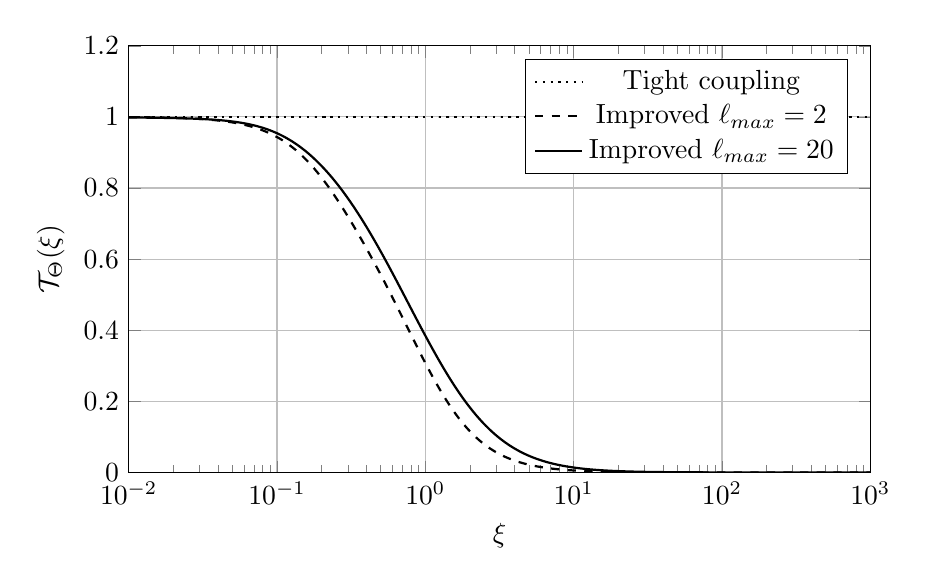
\begin{tikzpicture}
\begin{axis}[
    width=11cm, height=7cm,
    xlabel={$\xi$},
    ylabel={$\mathcal{T}_\Theta(\xi)$},
    xmin=1e-2, xmax=1e3,
    ymin=0, ymax=1.2,
    legend pos=north east,
    grid=major,
    domain=1e-2:1e3,
    samples=300,
    xmode=log
]
% Tight coupling (constant)
\addplot[thick, dotted, domain=1e-2:1e3] {1};
\addlegendentry{Tight coupling}

% Improved transfer function
\addplot[thick, dashed ,domain=1e-2:1e3] {(1+9.47*x*x+1.93*x*x*x*x)/(1+15.87*x^2+20*x^4+3.43*x^6)};
\addlegendentry{Improved $\ell_\text{max}=2$}
\addplot[thick, domain=1e-2:1e3] {(1+4.48*x+91*x*x)/(1+4.64*x+90.2*x^2+100*x^3+55*x^4)};
\addlegendentry{Improved $\ell_\text{max}=20$}

\end{axis}
\end{tikzpicture}
\caption{Comparison of the tight coupling transfer functions $\mathcal{T}_\Theta(\xi)$ and the improved one. Recall that $\xi \defeq k/(n_e\sigma_T a)$. We can appreciate how the improved functions recover the tight coupling limit at early times ($\xi\ll1$) while they vanish at the scale of the mean free path of photons ($\xi\gg1$).}
\label{fig:fight_coupling}
\end{figure}
\subsubsection{Dissipation in the y-era}
Modes reentering the comoving Hubble horizon during the y-era ($z<10^4$ from Section \ref{sec:ThermalizationScales}) encounter a different physical scenario: indeed the damping caused by free-streaming neutrinos is now almost negligible, furthermore, in this era the radiation-matter transition occurs and therefore different heating rates must be computed. 

To differentiate between the modes that reenter during matter and radiation domination we can define $k_\text{eq}\defeq aH|_\text{eq}\sim 10^{-2}$Mpc$^{-1}$ and $k_{\mu y}\defeq aH|_{\mu y}\sim 10^{-1}$Mpc$^{-1}$: for $k_{\mu y}>k>k_\text{eq}$ gravitational waves have already crossed the horizon before equality but already in the y-era, while for $k<k_\text{eq}$ the crossing occurs during matter domination.\\ From Section \ref{sec:free_GW} we know that gravitational waves evolve differently in the two eras, according to equation \eqref{eq:free_GW_sol}. During the radiation dominated era the transfer function of primordial gravitational waves reads, imposing that for $k\tau\to0$ the solution must be regular\footnote{This requirement is needed since on super-Hubble scales the constant solution must be recovered. Indeed we recall that for $x\to0$ $j_n(x)\sim x^{n}/(2n+1)!!$ and $j_n(x)\sim -(2n+1)!!/x^{n}$.}, $ j_0(k\tau)$, which derivative
instead gives $-kj_1(k\tau)$. Inserting this derivative inside the heating rate \eqref{eq:HRI_tight} we finally find
\begin{equation}
    \frac{d}{dt}\frac{\Delta\rho_\gamma}{\rho_\gamma}\bigg|_T=\frac{8H^2}{45n_e\sigma_T}\int\frac{d^3k}{(2\pi)^3}{P}_T\mathcal{T}_h^{RD}\mathcal T_\Theta e^{-\Gamma_\gamma\tau},\qquad\text{with }\mathcal{T}_h^{RD}\defeq (k\tau)^2j_1^2(k\tau).
\end{equation} 
In the matter dominated era instead, the amplitude of gravitational waves, requiring regularity for $k\tau\to0$, evolves as $j_1(k\tau)/(k\tau)$.
However we shall note that this function cannot be used as a proper transfer function since, as we consider the super Hubble horizon limit, and so the amplitude become just a constant, the above does not converge to unity:
$$\frac{j_1(k\tau)}{k\tau}\xrightarrow{k\tau\to0}\frac{k\tau}{3!!k\tau}+\mathcal{O}\big((k\tau)^2\big)=\frac{1}{3},$$
which suggest that a factor $3$, as reported by Watanabe and Komatsu in \cite{Watanabe_2006}, should be added.  
We can now compute its derivative
$$\frac{d}{d\tau}\frac{j_1(k\tau)}{k\tau}=\frac{k^2\tau j_1'(k\tau)-kj_1(k\tau)}{(k\tau)^2}=k\frac{j_1(k\tau)-k\tau j_2(k\tau)-j_1(k\tau)}{(k\tau)^2}=-k \frac{j_2(k\tau)}{k\tau},$$
where we used the recursive relation $j'_n(x)=n j_n(x)-xj_{n+1}(x)$. We conclude that the appropriate heating rate for the dissipation of gravitational waves reentering the Hubble horizon in the matter dominated era is 
\begin{equation}
    \frac{d}{dt}\frac{\Delta\rho_\gamma}{\rho_\gamma}\bigg|_T=\frac{2H^2}{45n_e\sigma_T}\int\frac{d^3k}{(2\pi)^3}{P}_T\mathcal{T}_h^{MD}\mathcal T_\Theta e^{-\Gamma_\gamma\tau},\qquad\text{with }\mathcal{T}_h^{MD}\defeq 9j_2^2(k\tau),
\end{equation}
where we must remove a factor $\times 4$ since during matter domination $a\propto \tau^2$ and therefore $H=2/(a\tau)$.
\section{Window functions}
While the information on the primordial perturbations are contained in the power spectrum, all the interactions occurring in the plasma can be encoded by the so-called the \textbf{window function}. In general, this means that the amplitude of a distortion can be expressed as
\begin{equation}\label{eq:window_function}
    a=\int\frac{d^3k}{(2\pi)^3} P_\delta(k) W_a(k)=\int\frac{dk}{k} \mathcal P_\delta(k) W_a(k) ,
\end{equation}
where $W_a(k)$ is the window function of the distortion $a$. This decomposition allows us to better understand at which scales perturbation dissipation more efficiently sources distortions. Inserting the heating rate we obtained in the previous section in the integral \eqref{eq:SD_amplitude_branching}, we find the actual full expression for the $\mu$-distortion generated by primordial gravitational waves
$$\mu=1.4\int_{0}^\infty dz\frac{8H^2}{45 n_e\sigma_T}\int_0^\infty\frac{k^2dk}{2\pi^2}\mathcal P_T(k)\mathcal T_h(k\tau)\mathcal T\Big(\tfrac{k}{n_e\sigma_ta}\Big)e^{-\Gamma_\gamma\tau}\mathcal{J}_\mu(z),$$
where $\mathcal{J}_\mu(z)$ is the branching ratio and $\mathcal T_h$ must change with $z$, as we explained in the last section.
This expression shows that, by inverting the order of integration, the window function of the $\mu$-distortions reads
\begin{align*}
    W_\mu(k)=1.4\int_{0}^\infty dz\frac{8H^2}{45 n_e\sigma_T}\mathcal T_h(k\tau)&\mathcal T\Big(\tfrac{k}{n_e\sigma_ta}\Big)e^{-\Gamma_\gamma\tau}\times\\&\times
    \begin{cases}
        e^{-(z/z_{\text{th}})^{5/2}}\Theta_H(z-z_{\mu y})\\
        e^{-(z/z_{\text{th}})^{5/2}}\Bigg\{1-\exp\bigg[-\big(\frac{1+z}{5.8\times10^4}\big)^{1.88}\bigg]\Bigg\}
    \end{cases},
\end{align*}
where we included two approximate expressions for the branching ratios and we recall that $z_\text{th}\approx 2\times 10^6$ and $z_{\mu y}\approx 5\times 10^4$.\\
The first branching ratio, that has been used in the work of Chluba et al. \cite{Chluba_tens_diss}, is obtained considering a sharp $\mu$-y transition \eqref{eq:BR_soft} while the latter takes into account that such transition is not instantaneous \eqref{eq:BR_soft_soft}. A comparison between the two resulting window functions is shown in Figure \ref{fig:mu_window}: as we can see, using the second branching ratio the window function covers a wider range of scales, reaching much bigger scales of the order of $k\sim10^{-5}$ Mpc$^{-1}$. On the other hand the small scale behavior remains the same, reaching the scales of $k\sim10^{8}$ Mpc$^{-1}$ still sourcing non-negligible $\mu$-distortions. The new contribution to the window function comes from the energy deposited in the plasma during the $\mu$-y transition, when both distortions can be sourced.
\begin{figure}
    \centering
\begin{tikzpicture}
  \begin{axis}[
      grid=major,
      xmode=log,
      ymode=log,
      xlabel={$k$ [1/Mpc]},
      ylabel={$W_\mu(k)$},
      width=12cm, height=8cm,
      legend pos = south east,
        xmax = 1e11, xmin = 1e-7,
      ymax = 1e-4, ymin = 1e-18
  ]
    % Load and plot from the external file
    \addplot [gray, smooth, thick] table {CMB/mu_Window_sharp.dat};
    \addlegendentry{J. Chluba - Sharp transition}
    \addplot [thick, smooth] table {CMB/mu_Window_soft.dat};
    \addlegendentry{Smooth $\mu$-y transition}
  \end{axis}
\end{tikzpicture}
\caption{Plot of the window function of the $\mu$ distortion sourced by the dissipation of primordial gravitational waves. A comparison between the window function obtained by J. Chluba in \cite{Chluba_tens_diss} and the one we obtained with a smooth $\mu$-y transitioning branching ratio is shown.}
\label{fig:mu_window}
\end{figure}

The window function for the y-distortion is instead obtained in the same way using instead the branching ratios corresponding to the y-distortions:
\begin{align*}
    W_y(k)=\frac14\int_{0}^\infty dz\frac{8H^2}{45 n_e\sigma_T}\mathcal T_h(k\tau)&\mathcal T\Big(\tfrac{k}{n_e\sigma_ta}\Big)e^{-\Gamma_\gamma\tau}\times
    \begin{cases}
        \Theta_H(z_{\mu y}-z)\\
        \bigg[1+\big(\frac{1+z}{6\times10^{4}}\big)^{2.58}\bigg]^{-1}
    \end{cases},
\end{align*}
Again, for the two branching ratios the window functions have been computed and are displayed in Figure \ref{fig:y_window}: we can appreciate that the smooth transition (black line) allows primordial gravitational waves that crossed back the comoving Hubble horizon at early times to contribute slightly more, since they are allowed to deposit energy already during the $\mu$-y transition. At large scales instead the two branching ratios give the same window functions.  

\begin{figure}
    \centering
\begin{tikzpicture}
  \begin{axis}[
      grid=major,
      xmode=log,
      ymode=log,
      xlabel={$k$ [1/Mpc]},
      ylabel={$W_y(k)$},
      width=12cm, height=8cm,
      legend pos = south west,
      xmax = 1e11, xmin = 1e-7,
      ymax = 1, ymin = 1e-19
  ]
    % Load and plot from the external file
    \addplot [gray, smooth, thick] table {CMB/y_Window_sharp.dat};
    \addlegendentry{Sharp $\mu$-y transition}
    \addplot [thick, smooth] table {CMB/y_Window_soft.dat};
    \addlegendentry{Smooth $\mu$-y transition}
  \end{axis}
\end{tikzpicture}
\caption{Plot of the window function of the y-distortion sourced by the dissipation of primordial gravitational waves. A comparison between the results obtained using the sharp transitioning (gray) and the smooth transitioning (black) branching ratio is showed.}
\label{fig:y_window}
\end{figure}
To conclude our analysis on the window functions, we would like to compare the results obtained by the dissipation of primordial gravitational waves and by the dissipation of scalar adiabatic perturbations. Following the results we found in Section \ref{sec:diss_scalar} we computed the corresponding window functions, which are shown in Figure \ref{fig:st_window}. From the plots, we can appreciate how the window functions associated with scalar perturbations are several orders of magnitude larger than those of primordial gravitational waves. This makes them much more likely to be detected by future experiments, such as PIXIE \cite{pixie}. On the other hand, the window function associated with primordial gravitational waves covers a much broader range of scales. Especially at small scales, while dissipation of scalar perturbations rapidly becomes negligible after $k\sim10^{4}$ Mpc$^{-1}$, primordial gravitational waves can still deposit energy in the plasma. This is most evident for really blue power spectra $n_t\sim1$.

\begin{figure}
    \centering
\begin{tikzpicture}
  \begin{axis}[
      grid=major,
      xmode=log,
      ymode=log,
      xlabel={$k$ [1/Mpc]},
      ylabel={$W(k)$},
      width=12cm, height=8cm,
      legend pos = south west,
      xmin = 1e-6, xmax = 1e9,
      ymax = 1e1 , ymin = 1e-13,
      xtick={1e-6, 1e-4, 1e-2, 1e0, 1e2, 1e4, 1e6, 1e8},
  ]
    % Load and plot from the external file
    \addplot [smooth, thick] table {CMB/mu_Window_soft.dat};
    \addlegendentry{$\mu$ Tensors}
    \addplot [thick, smooth, dashed] table {CMB/scalar_Window_mu.dat};
    \addlegendentry{$\mu$ Scalars}
    \addplot [gray, smooth, thick] table {CMB/y_Window_soft.dat};
    \addlegendentry{y Tensors}
    \addplot [thick, smooth, gray, dashed] table {CMB/scalar_Window_y.dat};
    \addlegendentry{y Scalars}
  \end{axis}
\end{tikzpicture}
\caption{Comparison of the window functions of the $\mu$ and y-distortions sourced by the dissipation of primordial gravitational waves and scalar perturbations. While the window functions associated to scalar perturbations (dashed) are in general larger, primordial gravitational waves (solid lines) can produce distortions on a wider range of scales.}
\label{fig:st_window}
\end{figure}

\section{Theoretical \sout{analysis} (maybe predictions) of the distortions}

At this stage we are able to produce theoretical predictions on the spectral distortions generated by the dissipation of primordial gravitational waves. To obtain these results we modified the \emph{distortion} module of \texttt{\texttt{CLASS}} so that the heating rate we obtained is computed numerically and then used by \texttt{\texttt{CLASS}} to calculate the spectral distortions amplitudes.


To begin with, we tried to reproduce the results that Chluba et al. obtained in \cite{Chluba_tens_diss}: this was initially used as a benchmark to understand whether our implementation ed correctly.
\begin{table}[b]
\begin{tabular}{llllll}
\hline
                                                                                                                   &                    & Chluba et al.       & Sharp tr.    & Smooth tr.  & Exact \\
\hline
\multirow{3}{*}{\begin{tabular}[c]{@{}l@{}}$\mathcal A_T=2.2\times10^{-10}$\\ $k_0=0.05$ Mpc$^{-1}$\end{tabular}}  & $n_t=0$            & $1.8\times10^{-14}$ & $1.8\times10^{-14}$ & $2.7\times10^{-14}$& $3.7\times10^{-14}$ \\
                                                                                                                   & $n_t=0.36$         & $3.7\times10^{-13}$ & $3.6\times10^{-13}$ & $4.0\times10^{-13}$& $5.0\times10^{-13}$ \\
                                                                                                                   & $n_t=1$            & $1.9\times10^{-9}$  & $1.8\times10^{-9}$  & $1.8\times10^{-9}$& $1.9\times10^{-9}$  \\

\hline
\multirow{3}{*}{\begin{tabular}[c]{@{}l@{}}$\mathcal A_T=2.4\times10^{-10}$\\ $k_0=0.002$ Mpc$^{-1}$\end{tabular}} & $n_t=0$            & $1.9\times10^{-14}$ & $1.9\times10^{-14}$ & $29\times10^{-14}$&$3.9\times10^{-14}$ \\
                                                                                                                   & $n_t=0.36$         & $1.3\times10^{-12}$ & $1.2\times10^{-12}$ & $1.4\times10^{-12}$ & $1.7\times10^{-12}$ \\
                                                                                                                   &$n_t=1$             & $5.3\times10^{-8}$ & $4.9\times10^{-8}$  & $4.9\times10^{-8}$ & $5.0\times10^{-8}$    \\                 
\hline
\end{tabular}
\caption{$\mu$-distortions amplitudes computed for different values of the spectral index $n_t=\{0,0.36,1\}$ and for two set of power spectrum amplitudes and pivot scale. The last columns compare the amplitudes obtained in \cite{Chluba_tens_diss} with our results. Results obtained both a sharp and smooth $\mu$-y transitioning and the exact branching ratios are reported.}
\label{tab:chluba_comp}
\end{table}
From Table \ref{tab:chluba_comp} we can see that we were able to reproduce (column \emph{Sharp tr.}) the same results obtained by Chluba et al. in \cite{Chluba_tens_diss}, using the same branching ratios. When the smooth $\mu$-y transition is considered instead the amplitudes increase and almost double using exact branching ratios computed through the Green's function method (Section \ref{sec:branching_ratios}). Note that this effect is evident for nearly scale invariant spectra, remaining a subdominant effect for blue tilted ones: this happens because blue tilted power spectra correspond to less excited modes that reenter the comoving Hubble horizon at later times, such as during the $\mu$-y transition.\\ The same results are shown in Figure \ref{fig:mu_amplitudes} but for all the spectral indexes ranging from 0 to 1: from this plot we can better appreciate how for nearly scale invariant power spectra perturbation dissipation during the $\mu$-y transition becomes more relevant. Finally, we can observe that only for very blue power spectra ($n_t>1$) the amplitude becomes comparable with those of Silk damping in the standard inflation scenario ($\mu\approx1.4\times10^{-8}$) \cite{Chluba_2x2}. However, this is quite in contrast with current constraints on the spectral index, which should be nearly scale invariant.

\begin{figure}
    \centering
\begin{tikzpicture}
  \begin{axis}[
      grid=major,
      ymode=log,
      xlabel={$n_t$},
      ylabel={$\mu$},
      width=12cm, height=8cm,
      legend pos = north west,
      xmin = -0.05, xmax = 1.1,
      ymin = 1e-14 , ymax =1e-8,
      %xtick={1e-6, 1e-4, 1e-2, 1e0, 1e2, 1e4, 1e6, 1e8},
  ]
    % Load and plot from the external file
    \addplot [smooth, thick] table {CMB/mu_exact.dat};
    \addlegendentry{Exact}
    \addplot [thick, smooth, dashed] table {CMB/mu_soft.dat};
    \addlegendentry{Smooth transitioning}
    \addplot [thick, smooth, dotted] table {CMB/mu_sharp.dat};
    \addlegendentry{Sharp transitioning}
    \addplot [only marks, thick] table {
    0 1.8e-14
    0.36 3.7e-13
    1 1.9e-9 
    };
    \addlegendentry{Points from Chluba et al.}
  \end{axis}
\end{tikzpicture}
\caption{Comparison of the amplitudes of $\mu$ distortions computed through our implementation of \texttt{\texttt{CLASS}} and the results (points on the plot) of Chluba et al. \cite{Chluba_tens_diss}. Different branching ratios results have been plotted as well. }
\label{fig:mu_amplitudes}
\end{figure}
We then conducted a similar comparison for y-distortions. From Figure \ref{fig:y_amplitudes} we can see that also for y-distortions, accounting for a non-instantaneous $\mu$-y transition, increases their amplitude.\\
Furthermore, although for scale invariant power spectra y-distortions are almost equal to $\mu$-distortions, the former grow much less as we increase the spectral index, resulting in bigger $\mu$-distortions already for $n_t>0.2$. For very blue power spectra $n_t\sim 1$ y-distortions are more than 3 order of magnitude smaller than the $\mu$ counterpart.  
\begin{figure}
    \centering
\begin{tikzpicture}
  \begin{axis}[
      grid=major,
      ymode=log,
      xlabel={$n_t$},
      ylabel={$y$},
      width=12cm, height=8cm,
      legend pos = north west,
      xmin = -0.05, xmax = 1.05,
      ymin = 5e-14 , ymax = 1e-10,
      %xtick={1e-6, 1e-4, 1e-2, 1e0, 1e2, 1e4, 1e6, 1e8},
  ]
    % Load and plot from the external file
    \addplot [smooth, thick] table {CMB/y_exact.dat};
    \addlegendentry{Exact}
    \addplot [thick, smooth, dashed] table {CMB/y_soft.dat};
    \addlegendentry{Smooth transitioning}
    \addplot [thick, smooth, dotted] table {CMB/y_sharp.dat};
    \addlegendentry{Sharp transitioning}
  \end{axis}
\end{tikzpicture}
\caption{Comparison of the amplitudes of y distortions computed through our implementation of \texttt{\texttt{CLASS}} for the different branching ratios. }
\label{fig:y_amplitudes}
\end{figure}
%    \begin{figure}[h]
%        \centering
%    \begin{tikzpicture}
%    \begin{axis}[
%        grid=major,
%        ymode=log,
%        xlabel={$r$},
%        ylabel={Amplitude},
%        width=12cm, height=8cm,
%        legend pos = north west,
%        xmin = 0, xmax = 1,
%        ymin = 1e-15 , ymax = 1e-11,
%        %xtick={1e-6, 1e-4, 1e-2, 1e0, 1e2, 1e4, 1e6, 1e8},
%    ]
%        % Load and plot from the external file
%        \addplot [thick, smooth] table[x index=0, y index=2] {CMB/mu_const.dat};
%        \addlegendentry{$\mu$-distortion}
%        \addplot [thick, smooth, gray] table[x index=0, y index=2] {CMB/y_const.dat};
%        \addlegendentry{y-distortion}
%    \end{axis}
%    \end{tikzpicture}
%    \caption{Comparison of the amplitudes of y distortions computed through our implementation of \texttt{\texttt{CLASS}} for the different branching ratios. }
%    \label{fig:mu_y_r}
%    \end{figure}
%
%    To conclude this first analysis we also studied the distortions that we would be sourced in presence of a primordial power spectrum which follows the consistency relation $r=-8n_t$. In Figure \ref{fig:mu_y_r} we can see that even when $r\sim1$ both the amplitudes of $\mu$ and y-distortions remain several orders of magnitude smaller than those sourced by scalar perturbations.

\subsection{Lognormal bump}
We have noted that considering the simplest inflation models, which we know to predict a power law primordial power spectrum both for scalar and tensor perturbations, it would  be very hard to detect any spectral distortion sourced by gravitational waves since it would be overshadowed by those produced by scalar perturbations. However, current constraints on the power spectrum of primordial gravitational waves are obtained from CMB anisotropies and these constraints could become not valid at different scales. This allows for the possibility of considering bumps in the power spectrum which make more excited only the modes that are relevant for our spectral distortions without spoiling current CMB measures.

As we discussed in Section \ref{sec:primordial_PS}, bumps can be modelled using a \textbf{lognormal} \eqref{eq:lognormal} function. For our analysis we therefore summed the lognormal bump at the pivot scale $K_\text{pk}=10$ Mpc$^{-1}$, which is in the middle of the window function of $\mu$ distortions, to the usual power law. For the power law we used $r=0.036$, which matches the upper bound set by BICEP/Kek\cite{Ade_2021}, and a tilt which satisfies the consistency relation $n_t=-r/8$, however slightly changes of these parameters will not influence our results until the power spectrum remains nearly scale invariant. 

To begin with, we studied which set of parameters are able to produce distortions of the order of $10^{-8}$: as it is shown in Figure \ref{fig:lognormal_res} at these scales already a tiny bump can push the distortions at the same order of magnitude of those produced by Silk damping. Considering a narrow bump ($\sigma_\text{bump}\sim0.1$) when $\mathcal{A}_\text{bump}\sim 10^{-2}$ we produce distortions $\mu\sim10^{-8}$, on the other hand bumps that are even slightly broader can produce similar distortions even though they are smaller: $\mathcal{A}_\text{bump}\sim 10^{-3}$ for $\sigma_\text{bump}\sim0.3$ and $\mathcal{A}_\text{bump}\sim 3\times10^{-4}$ for $\sigma_\text{bump}\sim1$. 

\begin{figure}[h!]
    \centering
\begin{tikzpicture}
  \begin{axis}[
      grid=major,
      ymode=log,
      xmode=log,
      xlabel={$\mathcal A_\text{bump}$},
      ylabel={$\mu$},
      width=15cm, height=8cm,
      legend pos = north west,
      legend style={font=\scriptsize},
      xmin = 1e-4, xmax = 1e-2,
      %ymin = 1e-13 , ymax = 1e-10,
      %xtick={1e-6, 1e-4, 1e-2, 1e0, 1e2, 1e4, 1e6, 1e8},
  ]

   \addplot[smooth, thick, green] table[col sep=space, x index=0,  y index = 1] {CMB/Lognormal/tensor_mu_aln@sigma1.000e-01.dat}; \addlegendentry{$\sigma_\text{bump}=0.1$}
    \addplot[smooth, thick, orange] table[col sep=space, x index=0,  y index = 1] {CMB/Lognormal/tensor_mu_aln@sigma1.778e-01.dat}; \addlegendentry{ $\sigma_\text{bump}=0.18$}
    \addplot[smooth, thick, red] table[col sep=space, x index=0,  y index = 1] {CMB/Lognormal/tensor_mu_aln@sigma3.162e-01.dat}; \addlegendentry{$\sigma_\text{bump}=0.31$}
    \addplot[smooth, thick, black] table[col sep=space, x index=0,  y index = 1] {CMB/Lognormal/tensor_mu_aln@sigma5.623e-01.dat}; \addlegendentry{$\sigma_\text{bump}=0.56$}
    \addplot[smooth, thick, blue] table[col sep=space, x index=0,  y index = 1] {CMB/Lognormal/tensor_mu_aln@sigma1.000e+00.dat}; \addlegendentry{$\sigma_\text{bump}=1$}   
    
  \end{axis}
\end{tikzpicture}
\caption{Amplitudes of $\mu$-distortions with a lognormal bump at $k_\text{pk}=10$Mpc$^{-1}$ as a function of the height of the bump. Different curves represent different width of the bump. }
\label{fig:lognormal_res}
\end{figure}

\begin{figure}[h!]
    \centering
\begin{tikzpicture}
  \begin{axis}[
      grid=major,
      ymode=log,
      xmode=log,
      xlabel={$\sigma_{bump}$},
      ylabel={$\mu$},
      width=15cm, height=8cm,
      legend pos = north east,
      legend style={font=\scriptsize},
      xmin = 5e-1, xmax = 1e2,
      %ymin = 1e-13 , ymax = 1e-10,
      %xtick={1e-6, 1e-4, 1e-2, 1e0, 1e2, 1e4, 1e6, 1e8},
  ]

    \addplot[smooth, thick, blue] table[col sep=space, x index=0,  y index = 1] {CMB/Plateau/tensor_mu_sigma@aln1.000e-03.dat}; \addlegendentry{PGW $\mathcal{A}_\text{bump}=1\times10^{-3}$}   
    \addplot[smooth, thick, green] table[col sep=space, x index=0,  y index = 1] {CMB/Plateau/tensor_mu_sigma@aln5.623e-04.dat}; \addlegendentry{PGW $\mathcal{A}_\text{bump}=5\times10^{-4}$}
    \addplot[smooth, thick, orange] table[col sep=space, x index=0,  y index = 1] {CMB/Plateau/tensor_mu_sigma@aln1.778e-04.dat}; \addlegendentry{PGW $\mathcal{A}_\text{bump}=2\times10^{-4}$}
    \addplot[smooth, thick, red] table[col sep=space, x index=0,  y index = 1] {CMB/Plateau/tensor_mu_sigma@aln1.000e-04.dat}; \addlegendentry{PGW $\mathcal{A}_\text{bump}=1\times10^{-4}$}
    

    
    \addplot[smooth, thick, dashed, blue] table[col sep=space, x index=0,  y index = 1] {CMB/Plateau/scalar_mu_sigma@aln1.000e-03:.3e.dat}; \addlegendentry{Scalar $\mathcal{A}_\text{bump}=1\times10^{-3}$}
    \addplot[smooth, thick, dashed, green] table[col sep=space, x index=0,  y index = 1] {CMB/Plateau/scalar_mu_sigma@aln1.778e-04:.3e.dat}; \addlegendentry{Scalar $\mathcal{A}_\text{bump}=2\times10^{-4}$}
     \addplot[smooth, thick, dashed, orange] table[col sep=space, x index=0,  y index = 1] {CMB/Plateau/scalar_mu_sigma@aln5.623e-06:.3e.dat}; \addlegendentry{Scalar $\mathcal{A}_\text{bump}=5\times10^{-6}$}
    \addplot[smooth, thick, dashed, red] table[col sep=space, x index=0,  y index = 1] {CMB/Plateau/scalar_mu_sigma@aln1.000e-06:.3e.dat}; \addlegendentry{Scalar $\mathcal{A}_\text{bump}=1\times10^{-6}$}
    
  \end{axis}
\end{tikzpicture}
\caption{Comparison of the amplitudes of $\mu$-distortions with a lognormal bump as a function of the width of the bump. Dotted lines represent the distortions produced by scalar perturbations ($k_\text{pk}=1000$Mpc$^{-1}$), while solid lines represent distortions sourced by gravitational waves ($k_\text{pk}=10$Mpc$^{-1}$). }
\label{fig:ln_plateau}
\end{figure}

We then studied the behavior of the distortions as we increase the width of the bump until it covers the full range of scales of the window function of $\mu$-distortions. For this analysis it is important to keep in mind that, considering the lognormal bump \eqref{eq:lognormal}, the interval of scales covered by $n\sigma_\text{bump}$ grows exponentially as
$$k=k_\text{pk}e^{\pm n\sigma_\text{bump}}\approx k_\text{pk}10^{\pm n\sigma_\text{bump}\times 0.43},$$
which give us a rough idea of the range of scales covered by the bump. In Figure \ref{fig:ln_plateau} it is shown this behavior: for small values of $\sigma_\text{bump}$ the distortion amplitudes keep increasing until we reach $\sigma_\text{bump}\sim10$, from this point the growth stops and a plateau starts in the graph of $\mu$. Indeed, for $\sigma_\text{bump}\sim10$, already the 1-$\sigma_\text{bump}$ interval covers $k\sim 10^{-3}-10{5}$ Mpc$^{-1}$, which matches our window function (Figure \ref{fig:mu_window}). Note that in this case, even bumps which height is quite small ($10^{-3}-10^{-4}$) are able to plateau over $\mu=10^{-8}$.\\
To conclude this analysis we also computed the distortions produced by dissipation of scalar perturbation including a bump at scale $k=1000$ Mpc$^{-1}$. A totally analogous behavior is shown also in this case (dotted lines in Figure \ref{fig:ln_plateau}). However, Silk damping is able to produce distortions that are several order of magnitude ($\sim10^5$) bigger even when using bumps that are way smaller (for $\mathcal A_\text{bump}=10^{-6}$ the plateau sits at $\mu\sim 10^{-5}$).

\begin{figure}[]
    \centering
\begin{tikzpicture}
  \begin{axis}[
      grid=major,
      ymode=log,
      xmode=log,
      xlabel={$\sigma_{bump}$},
      ylabel={Amplitude},
      width=15cm, height=8cm,
      legend pos = south east,
      legend style={font=\scriptsize},
      xmin = 1e-2, xmax = 1e3,
      %ymin = 1e-13 , ymax = 1e-10,
      %xtick={1e-6, 1e-4, 1e-2, 1e0, 1e2, 1e4, 1e6, 1e8},
  ]

    \addplot[smooth, thick, blue] table[col sep=space, x index=0,  y index = 1] {CMB/Plateau/mu_sigma@aln1.000e-02.dat}; \addlegendentry{$\mu$ $\mathcal{A}_\text{bump}=1\times10^{-2}$}   
    \addplot[smooth, thick, green] table[col sep=space, x index=0,  y index = 1] {CMB/Plateau/mu_sigma@aln1.000e-03.dat}; \addlegendentry{$\mu$ $\mathcal{A}_\text{bump}=1\times10^{-3}$}
    \addplot[smooth, thick, red] table[col sep=space, x index=0,  y index = 1] {CMB/Plateau/mu_sigma@aln1.000e-04.dat}; \addlegendentry{$\mu$ $\mathcal{A}_\text{bump}=1\times10^{-4}$}
    
    

    
    \addplot[smooth, thick, blue, dashed] table[col sep=space, x index=0,  y index = 1] {CMB/Plateau/y_sigma@aln1.000e-02.dat}; \addlegendentry{y $\mathcal{A}_\text{bump}=1\times10^{-2}$}   
    \addplot[smooth, thick, green, dashed] table[col sep=space, x index=0,  y index = 1] {CMB/Plateau/y_sigma@aln1.000e-03.dat}; \addlegendentry{y $\mathcal{A}_\text{bump}=1\times10^{-3}$}
    \addplot[smooth, thick, red, dashed] table[col sep=space, x index=0,  y index = 1] {CMB/Plateau/y_sigma@aln1.000e-04.dat}; \addlegendentry{y $\mathcal{A}_\text{bump}=1\times10^{-4}$}
    
  \end{axis}
\end{tikzpicture}
\caption{Comparison of the amplitudes of $\mu$-distortions  and y-distortions with a lognormal bump as a function of the width of the bump. For both the same bump is placed at $k_\text{pk}=10$Mpc$^{-1}$.}
\label{fig:muy_plateau}
\end{figure}

To conclude our analysis, we compared the $\mu$ and y amplitudes resulting from the same bump in the tensor power spectrum. As we can in see in Figure \ref{fig:muy_plateau}, both distortions starts with values in agreement with those we obtained for nearly scale invariant power spectra, then, as the width of the bump increases, they both grow in the same way and with similar values. However, when the bump saturates the window functions, while the $\mu$-distortions directly plateau, y-distortions rapidly increase to then plateau at a much higher value (roughly one order of magnitude more). This is due to the fact that when the bump reaches the largest scales ($k\sim10^{-4}$ Mpc$^{-1}$) the modes that reentered the comoving Hubble horizon during the y-era are excited as well, allowing for a sudden increase of the y-distortions amplitude. Please note that, these scenarios are out ruled by CMB anisotropies, since such large bumps would also affect the BB modes of CMB polarization. 